\chapter{Quick Revision: PE-EC802B - Industrial Automation and Control}

This document compiles high-density definitions, essential formulas, tuning tables, practicing diagrams, and a comprehensive database of solved exam one-liners across all 4 units for active recall.


\section{Section 1: Core Definitions to Memorize}

\subsection{Unit I: Sensors \& Actuators}
\begin{itemize}
  \item \textbf{Active Transducers:} Self-generating sensors that convert physical energy directly into electrical energy without requiring an external power source (e.g., Thermocouples, Piezoelectric crystals).
  \item \textbf{Passive Transducers:} Sensors that cause a change in electrical parameters ($R, L, C$) and require an auxiliary external electrical source to operate (e.g., RTDs, LVDTs, Strain Gauges).
  \item \textbf{LVDT (Linear Variable Differential Transformer):} A passive inductive transducer consisting of a primary coil and two series-opposing secondary coils. It measures linear displacement with infinite resolution by tracking the position of a moving ferromagnetic core.
  \item \textbf{Seebeck Effect:} The generation of an electromotive force (EMF) when two dissimilar metal junctions are held at different temperatures.
  \item \textbf{Gauge Factor (G):} A measure of the sensitivity of a strain gauge, representing the ratio of fractional change in resistance to longitudinal strain.
  \item \textbf{Back EMF ($E_b$):} The internal voltage induced in a DC motor's rotating armature that opposes the applied terminal voltage.
  \item \textbf{Motor Starters:} Devices that limit the high starting current of a motor (which occurs because Back EMF is zero at standstill) by inserting a variable series resistance.
  \item \textbf{Pneumatic Actuator:} An actuator that converts compressed air signals (standard $3\text{--}15\ \text{psi}$) into linear or rotary displacement.
  \item \textbf{Optoisolation:} The use of an optocoupler (LED + phototransistor) to transmit signals across an optical path, preventing high voltage transients on the field side from damaging the controller.
  \item \textbf{Calibration:} The process of comparing an instrument's output against a traceable reference standard of higher accuracy to detect deviations and establish correction bounds.
  \item \textbf{Systematic Errors:} Predictable, unidirectional measurement offsets caused by calibration errors, environmental changes, or parallax. They can be eliminated by calibration.
  \item \textbf{Random Errors:} Unpredictable variations caused by electrical noise or environmental fluctuations. They cannot be eliminated but are reduced statistically using the mean of multiple readings.
\end{itemize}

\subsection{Unit II: Controller Tuning}
\begin{itemize}
  \item \textbf{Servo Operation:} A control loop operating condition where the primary goal is to track a dynamically changing setpoint ($R(s)$).
  \item \textbf{Regulatory Operation:} A control loop operating condition where the primary goal is to keep the process variable constant by rejecting load disturbances ($D(s)$).
  \item \textbf{Self-Regulating System:} A process that naturally finds a new stable equilibrium following a step change in input without any controller intervention (e.g., gravity-drained liquid tank).
  \item \textbf{Non-Self-Regulating (Integrating) System:} A process that continuously drifts or ramps following a step input change until a physical limit is hit (e.g., pump-drained tank).
  \item \textbf{Dead-Time (Transport Lag):} The time delay between the application of an input signal and the first observable process response, modeled as $e^{-s T_d}$.
  \item \textbf{Proportional Band (PB):} The percentage of error required to drive the controller output from $0\%$ to $100\%$. Formulated as $PB = 100/K_c$.
  \item \textbf{Reset Windup:} The saturation of an Integral controller's output due to a persistent error, leading to large overshoot as the controller takes time to decrease its integrated value.
  \item \textbf{Noise Amplification:} A major limitation of Derivative controllers where high-frequency measurement noise is amplified by the derivative term ($\tau_D \frac{de}{dt}$), causing control valve wear.
\end{itemize}

\subsection{Unit III: Automation Systems}
\begin{itemize}
  \item \textbf{PLC (Programmable Logic Controller):} A rugged, solid-state industrial computer designed to monitor inputs, execute sequential program logic, and control field actuators.
  \item \textbf{PLC Scan Cycle:} The continuous execution cycle consisting of: (1) Read inputs to image table, (2) Solve ladder program sequentially, (3) Perform diagnostics/comm, and (4) Update output terminals.
  \item \textbf{DCS (Distributed Control System):} A control architecture where autonomous controllers (LCUs) are distributed throughout a plant, coordinated via a high-speed system bus, eliminating a single point of failure.
  \item \textbf{SCADA (Supervisory Control and Data Acquisition):} A software-hardware system designed for supervisory control and real-time telemetry data collection from geographically dispersed remote assets.
  \item \textbf{Master Terminal Unit (MTU):} The central host server in a SCADA system that queries remote field stations, stores databases, and drives operator HMIs.
  \item \textbf{Remote Terminal Unit (RTU):} A rugged remote microcontroller deployed at SCADA field sites to collect sensor data, format telemetry, and execute supervisory commands.
  \item \textbf{Globe Valve:} A linear control valve with a spherical body and baffle plate, widely used for throttling fluid pressure and flow rate control.
  \item \textbf{Valve Seat Ring:} The stationary seat ring fixed inside a control valve. When the plug is fully connected to the seat, the valve is fully closed.
\end{itemize}

\subsection{Unit IV: Advanced Control Techniques}
\begin{itemize}
  \item \textbf{Feedforward Control:} A proactive control strategy where load disturbances are measured and corrected for before they affect the process variable.
  \item \textbf{Ratio Control:} A control system designed to maintain a constant ratio between two flow streams ($R = F_C / F_W$).
  \item \textbf{Cascade Control:} A nested loop configuration containing a primary (outer) Master loop and a fast-acting secondary (inner) Slave loop.
  \item \textbf{Split-Range Control:} A loop configuration where a single controller output is split to drive two or more control valves sequentially (e.g. heating and cooling).
  \item \textbf{Override (Selective) Control:} A safety loop where multiple controllers share a single control valve through High/Low Selectors to protect equipment during limit crossings.
  \item \textbf{Adaptive Control:} A control system that adjusts its gains dynamically in real-time to compensate for process gain drift.
  \item \textbf{Internal Model Control (IMC):} A control structure running a process model in parallel with the actual plant to isolate disturbances ($d = Y - \tilde{Y}$) and feed them back to the controller.
\end{itemize}


\section{Section 2: Key Formulas \& Parameter Tables}

\subsection{1. Transducer \& Actuator Physics}
\begin{itemize}
  \item \textbf{Thermocouple EMF:}
\end{itemize}
  \[ E = a(T_{hot} - T_{cold}) + b(T_{hot} - T_{cold})^2 \]
\begin{itemize}
  \item \textbf{Cold Junction Compensation:}
\end{itemize}
  \[ V_{net} = V_{raw} + V_{comp} \]
\begin{itemize}
  \item \textbf{RTD Resistance:}
\end{itemize}
  \[ R_T = R_0 [1 + \alpha(T - T_0)] \]
\begin{itemize}
  \item \textbf{Strain Gauge Gauge Factor (G):}
\end{itemize}
  \[ G = \frac{\Delta R/R}{\Delta L/L} = 1 + 2\nu + \frac{\Delta\rho/\rho}{\Delta L/L} \]
  where $\nu$ is Poisson's ratio, and $\frac{\Delta\rho}{\rho}$ is the piezoresistive effect.
\begin{itemize}
  \item \textbf{Ultrasonic Distance (ToF):}
\end{itemize}
  \[ D = \frac{v \times t}{2} \]
  where $v$ is the speed of sound ($343\ \text{m/s}$ at $20^\circ\text{C}$), and $t$ is the time-of-flight.
\begin{itemize}
  \item \textbf{DC Motor Armature Current \& Back EMF:}
\end{itemize}
  \[ E_b = V - I_a R_a \implies I_{start} = \frac{V}{R_a} \quad (\text{since } E_b = 0 \text{ at } N=0) \]

\subsection{2. Controller Equations}
\begin{itemize}
  \item \textbf{Active Low-Pass Filter (LPF) Transfer Function \& Cut-off:}
\end{itemize}
  \[ H(s) = \frac{A_v}{1 + sRC}, \quad f_c = \frac{1}{2\pi RC} \]
\begin{itemize}
  \item \textbf{Active High-Pass Filter (HPF) Transfer Function \& Cut-off:}
\end{itemize}
  \[ H(s) = \frac{A_v sRC}{1 + sRC}, \quad f_c = \frac{1}{2\pi RC} \]
\begin{itemize}
  \item \textbf{Parallel PID Controller Transfer Function:}
\end{itemize}
  \[ G_c(s) = K_c \left[ 1 + \frac{1}{\tau_I s} + \tau_D s \right] \]
\begin{itemize}
  \item \textbf{Ideal Feedforward Controller:}
\end{itemize}
  \[ G_{ff}(s) = -\frac{G_d(s)}{G_v(s) G_p(s)} \]
\begin{itemize}
  \item \textbf{First-Order Padé Approximation of Dead Time:}
\end{itemize}
  \[ e^{-s T_d} \approx \frac{1 - \frac{T_d}{2} s}{1 + \frac{T_d}{2} s} \]


\subsection{3. Controller Tuning Tables}

\textbf{ZN Open-Loop (Process Reaction Curve) Tuning Table:}
\begin{itemize}
  \item Parameters: Dead time ($L$), Time constant ($T$).
\end{itemize}
\begin{table}[H]
\centering
\begin{tabular}{|p{\dimexpr 0.18\textwidth - 2\tabcolsep - 1.5\arrayrulewidth\relax}|p{\dimexpr 0.27\textwidth - 2\tabcolsep - 1.5\arrayrulewidth\relax}|p{\dimexpr 0.27\textwidth - 2\tabcolsep - 1.5\arrayrulewidth\relax}|p{\dimexpr 0.28\textwidth - 2\tabcolsep - 1.5\arrayrulewidth\relax}|}
\hline
Controller Type & Proportional Gain ($K_c$) & Integral Time ($\tau_I$) & Derivative Time ($\tau_D$) \\
\hline
\textbf{P} & $\frac{T}{L}$ & $-$ & $-$ \\
\hline
\textbf{PI} & $0.9 \frac{T}{L}$ & $3.3 L$ & $-$ \\
\hline
\textbf{PID} & $1.2 \frac{T}{L}$ & $2.0 L$ & $0.5 L$ \\
\hline
\end{tabular}
\end{table}

\textbf{ZN Closed-Loop (Ultimate Gain) Tuning Table:}
\begin{itemize}
  \item Parameters: Ultimate Gain ($K_u$), Ultimate Period ($P_u$).
\end{itemize}
\begin{table}[H]
\centering
\begin{tabular}{|p{\dimexpr 0.18\textwidth - 2\tabcolsep - 1.5\arrayrulewidth\relax}|p{\dimexpr 0.27\textwidth - 2\tabcolsep - 1.5\arrayrulewidth\relax}|p{\dimexpr 0.27\textwidth - 2\tabcolsep - 1.5\arrayrulewidth\relax}|p{\dimexpr 0.28\textwidth - 2\tabcolsep - 1.5\arrayrulewidth\relax}|}
\hline
Controller Type & Proportional Gain ($K_c$) & Integral Time ($\tau_I$) & Derivative Time ($\tau_D$) \\
\hline
\textbf{P} & $0.5 K_u$ & $-$ & $-$ \\
\hline
\textbf{PI} & $0.45 K_u$ & $\frac{P_u}{1.2}$ & $-$ \\
\hline
\textbf{PID} & $0.6 K_u$ & $0.5 P_u$ & $\frac{P_u}{8}$ \\
\hline
\end{tabular}
\end{table}

\textbf{Cohen-Coon PID Formulas (Quarter-Amplitude Decay):}
\begin{itemize}
  \item Parameters: Process Gain ($K_p$), Dead time ($L$), Time constant ($T$).
\end{itemize}
\[ K_c = \frac{1}{K_p} \frac{T}{L} \left[ \frac{4}{3} + \frac{L}{4T} \right], \quad \tau_I = L \left[ \frac{32 + 6(L/T)}{13 + 8(L/T)} \right], \quad \tau_D = L \left[ \frac{4}{11 + 2(L/T)} \right] \]

\subsection{4. Error Propagation}
\begin{itemize}
  \item \textbf{Addition or Subtraction ($X = x_1 \pm x_2$):}
\end{itemize}
  \[ \Delta X = \Delta x_1 + \Delta x_2 \quad (\text{absolute errors sum}) \]
\begin{itemize}
  \item \textbf{Multiplication or Division ($X = x_1 \cdot x_2$ or $X = x_1 / x_2$):}
\end{itemize}
  \[ \frac{\Delta X}{X} = \frac{\Delta x_1}{x_1} + \frac{\Delta x_2}{x_2} \quad (\text{relative errors sum}) \]


\section{Section 3: Diagrams to Practice Sketching}

Prepare to sketch these block architectures, response curves, and circuit schematics by hand:

\subsection{1. LVDT Electro-Mechanical Schematic (Unit I)}
Detailed diagram showing the primary and secondary series-opposing windings with a movable magnetic core.
\begin{figure}[H]
\centering
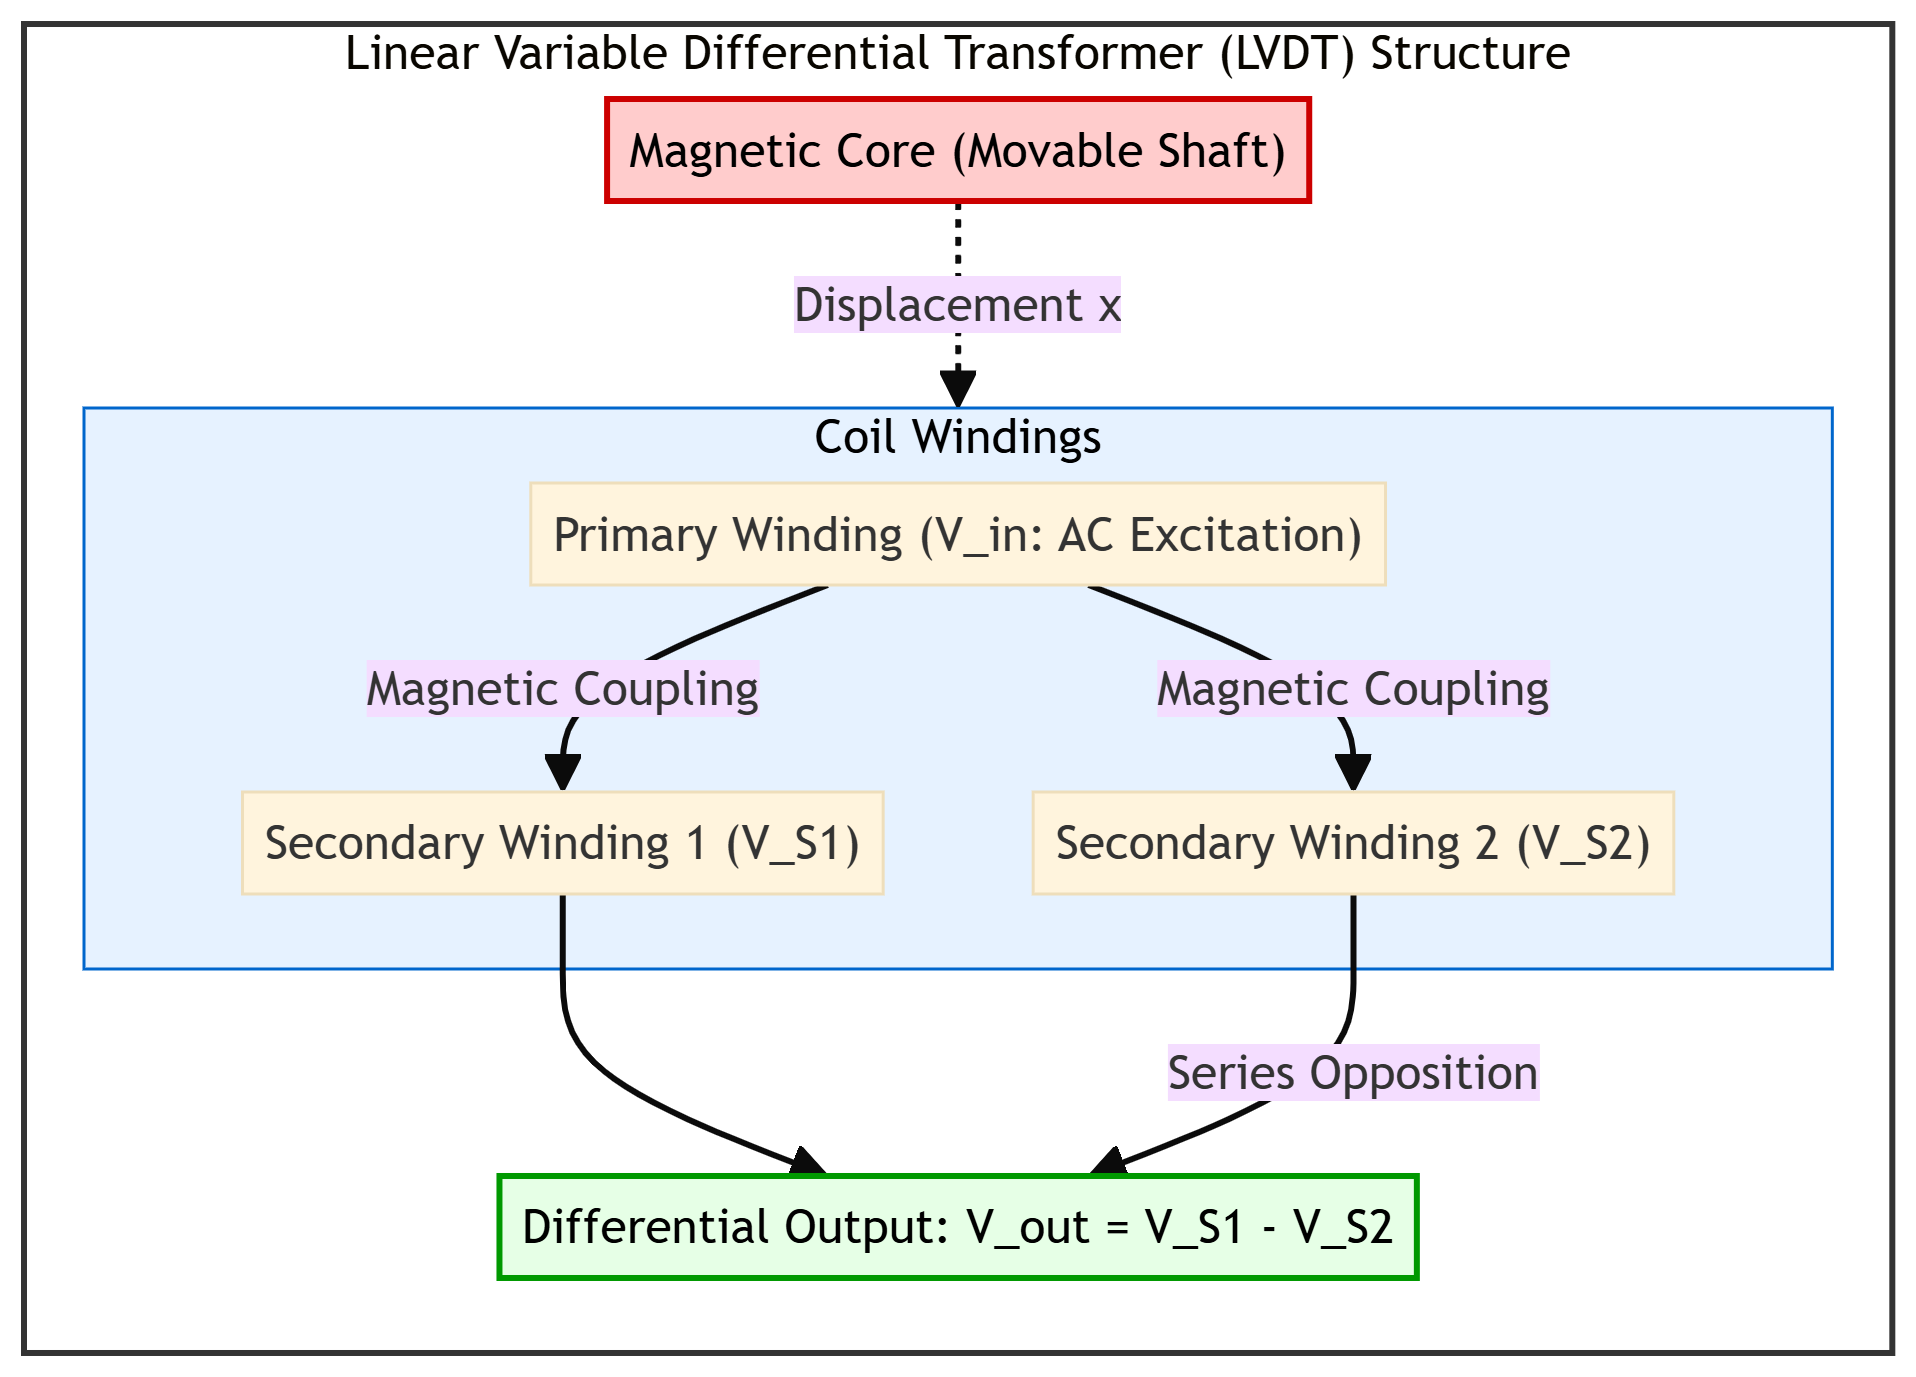
\includegraphics[width=0.75\textwidth,height=0.32\textheight,keepaspectratio]{../Images/chapter_01/lvdt_schematic.png}
\caption{LVDT Electro-Mechanical Schematic}
\end{figure}

\subsection{2. LVDT Transfer Characteristics (Unit I)}
Output voltage magnitude showing a linear response with a null residual voltage, and the $180^\circ$ phase shift through null.
\begin{figure}[H]
\centering
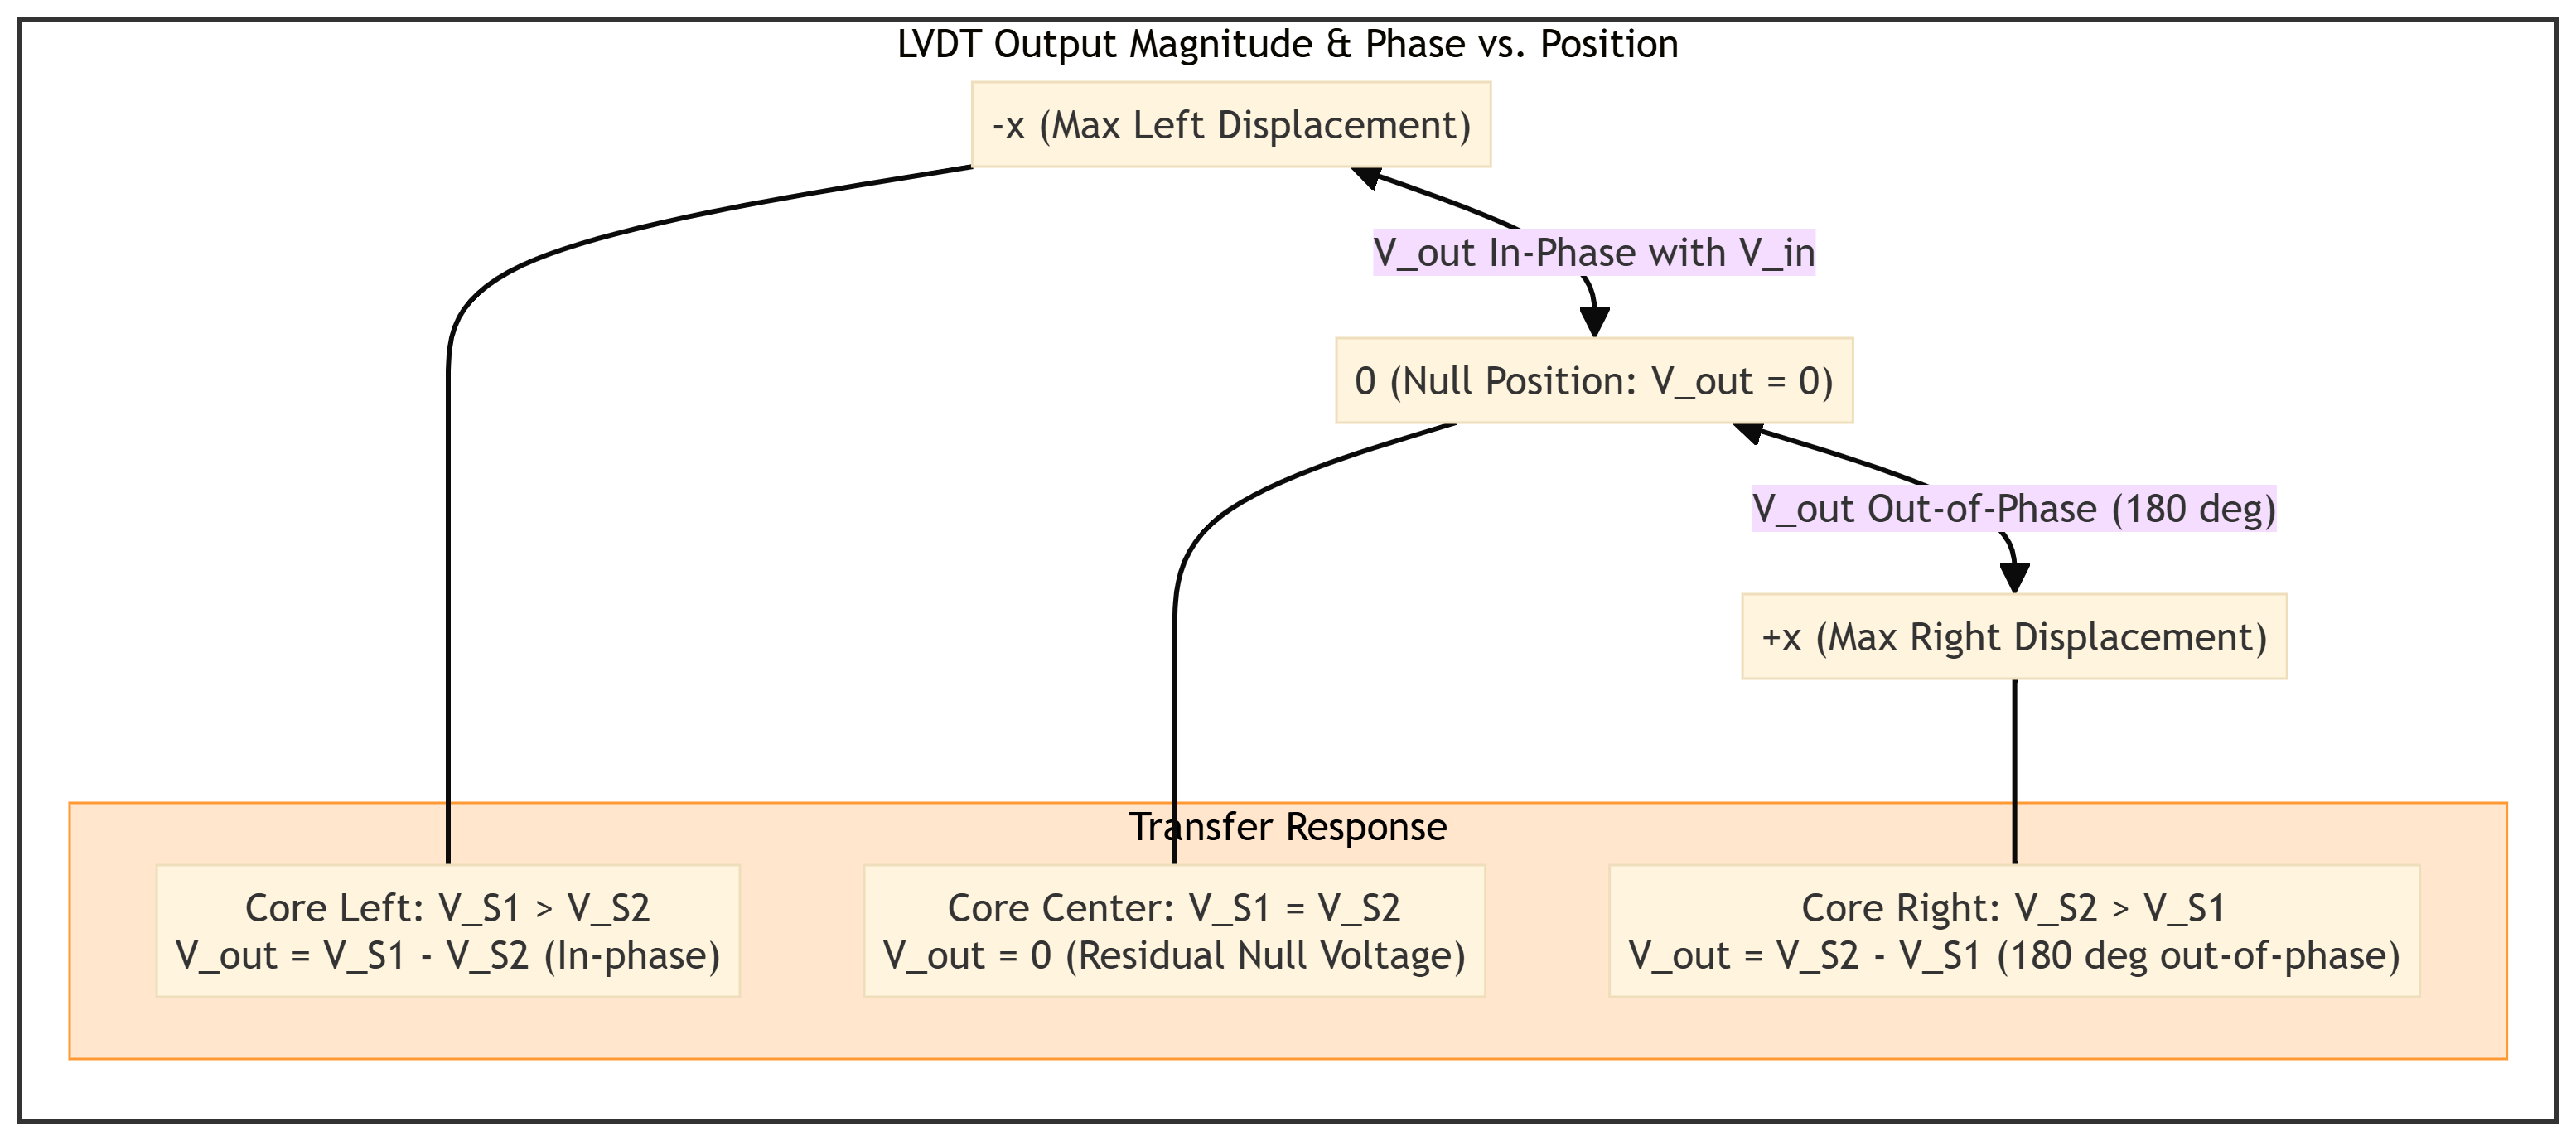
\includegraphics[width=0.75\textwidth,height=0.32\textheight,keepaspectratio]{../Images/chapter_01/lvdt_transfer_char.png}
\caption{LVDT Transfer Characteristics}
\end{figure}

\subsection{3. Thermocouple \& Cold Junction Compensation (Unit I)}
Circuit setup showing measuring and reference junctions with an active compensation bridge circuit.
\begin{figure}[H]
\centering
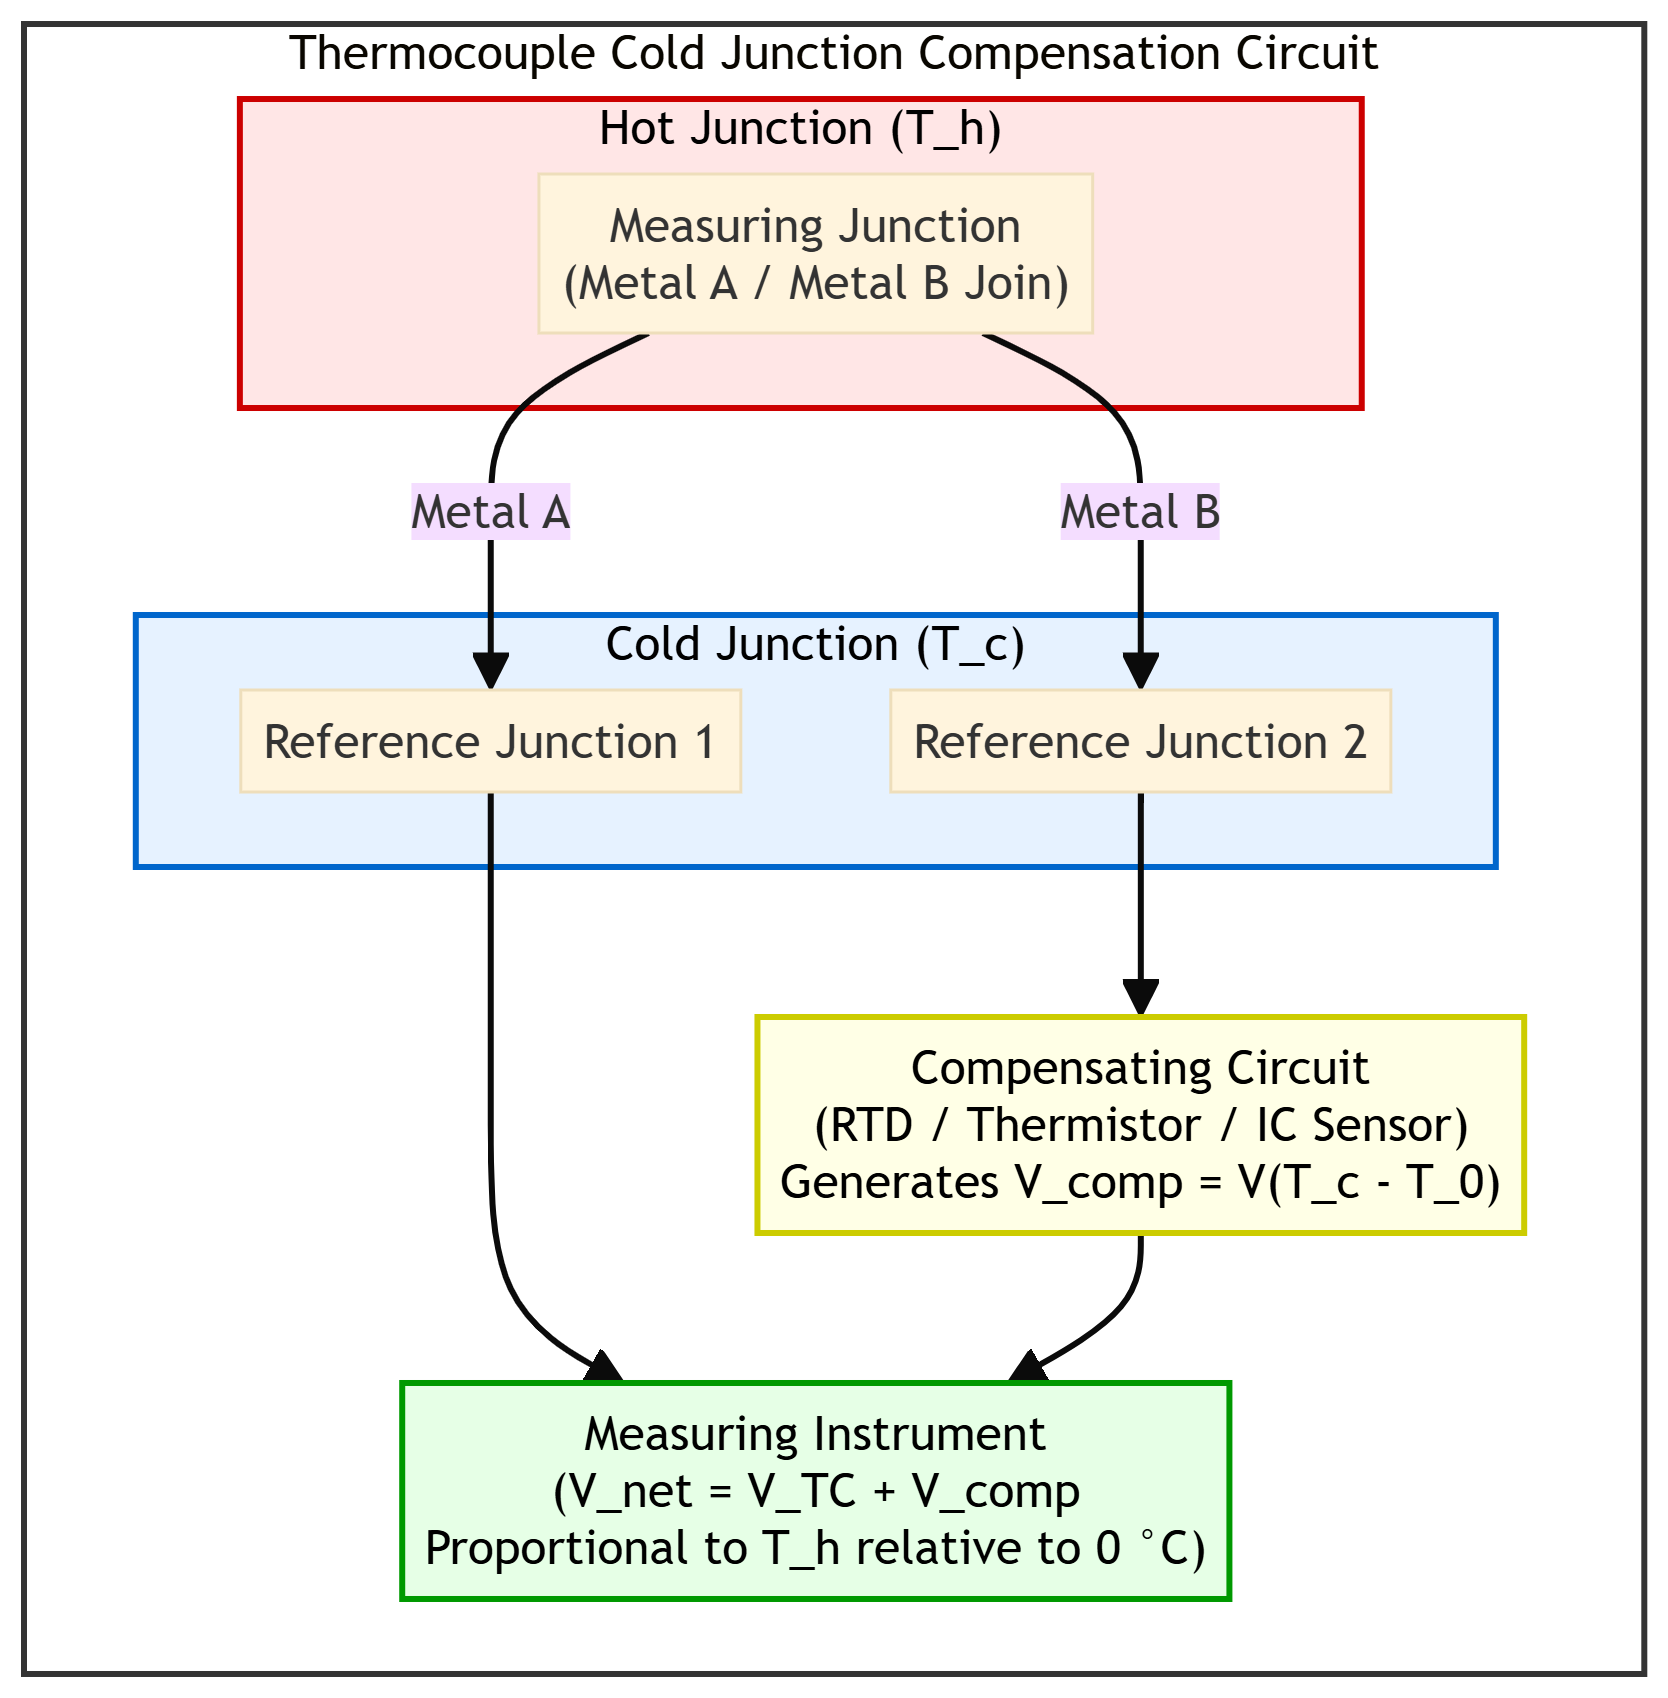
\includegraphics[width=0.75\textwidth,height=0.32\textheight,keepaspectratio]{../Images/chapter_01/thermocouple_compensation.png}
\caption{Thermocouple \& Cold Junction Compensation}
\end{figure}

\subsection{4. Pneumatic Spring-Diaphragm Actuator (Unit I)}
Mechanical assembly converting control air pressure ($3\text{--}15\ \text{psi}$) to linear stem displacement.
\begin{figure}[H]
\centering
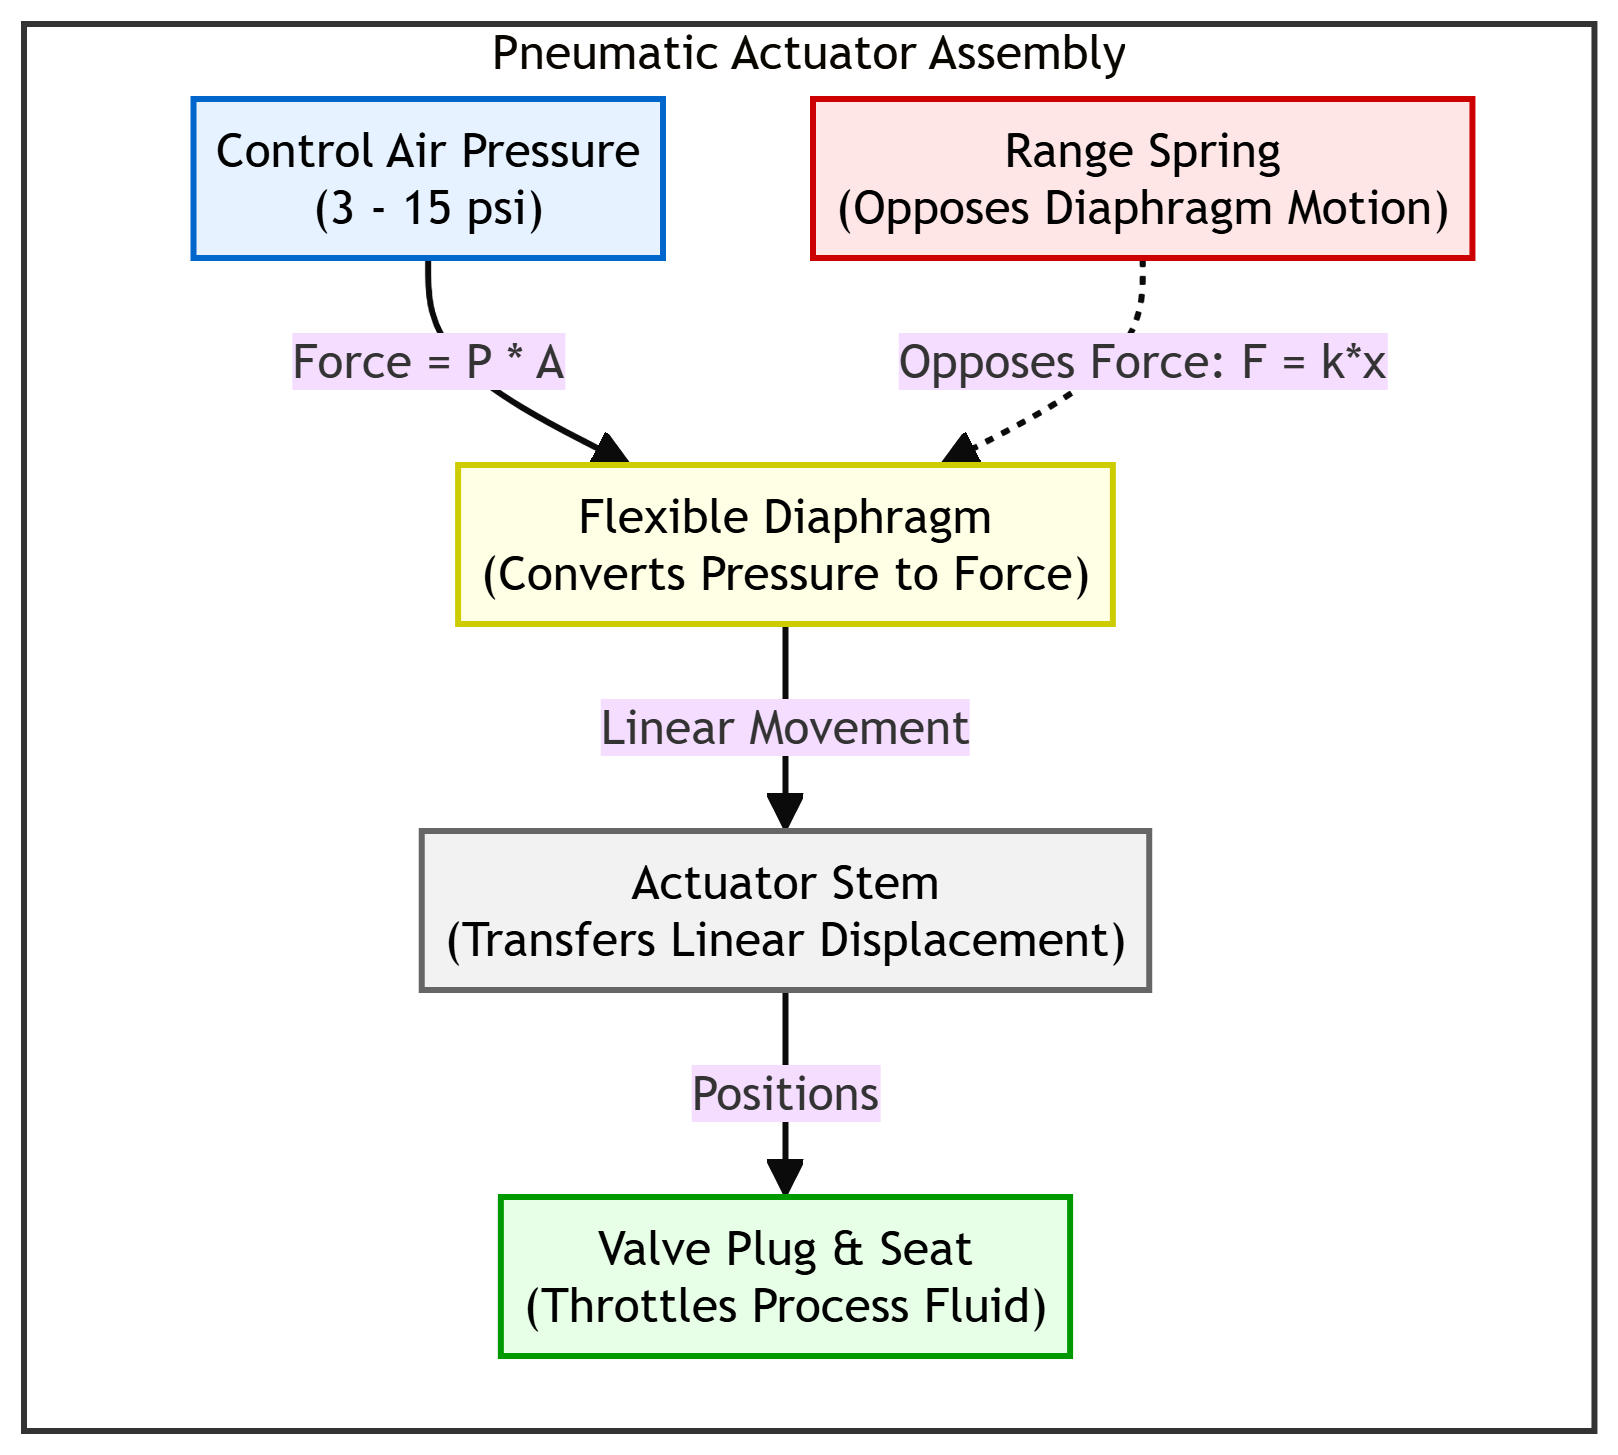
\includegraphics[width=0.75\textwidth,height=0.32\textheight,keepaspectratio]{../Images/chapter_01/pneumatic_actuator.png}
\caption{Pneumatic Spring-Diaphragm Actuator}
\end{figure}

\subsection{5. Signal Conditioning Flow (Unit I)}
The sequence of hardware stages processing a physical sensor variable into a digital signal.
\begin{figure}[H]
\centering
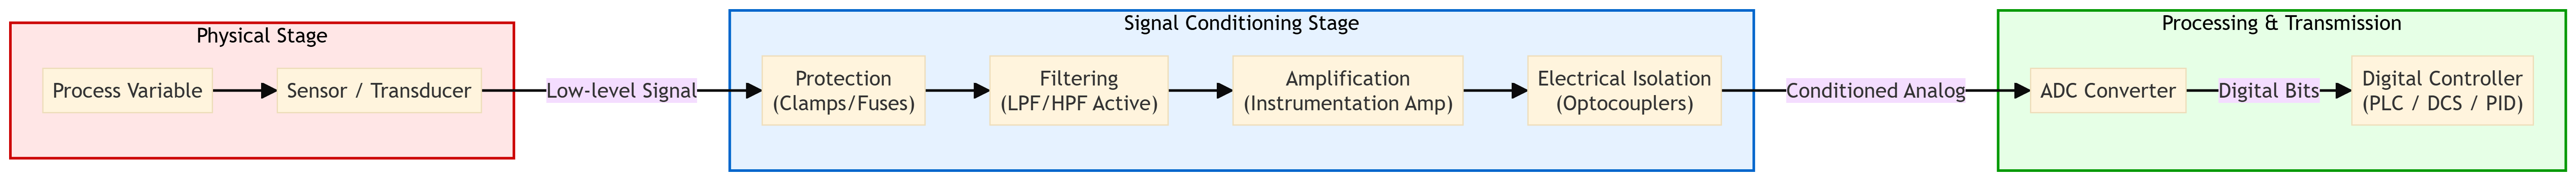
\includegraphics[width=0.75\textwidth,height=0.32\textheight,keepaspectratio]{../Images/chapter_01/signal_conditioning_block.png}
\caption{Signal Conditioning Functional Architecture}
\end{figure}

\subsection{6. Active Filters (Unit I)}
Operational amplifier circuits for low-pass and high-pass filtering.
\begin{figure}[H]
\centering
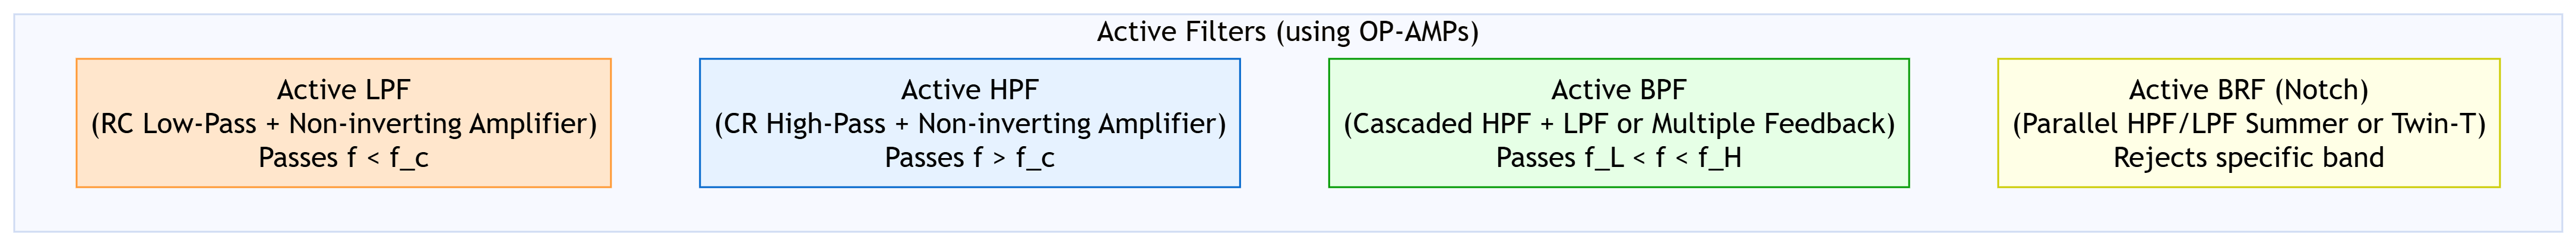
\includegraphics[width=0.75\textwidth,height=0.32\textheight,keepaspectratio]{../Images/chapter_01/opamp_filters.png}
\caption{Active Filter Circuit Topologies}
\end{figure}

\subsection{7. OP-AMP Parallel PID (Unit II)}
The physical summing op-amp schematic combining proportional, integral, and derivative paths.
\begin{figure}[H]
\centering
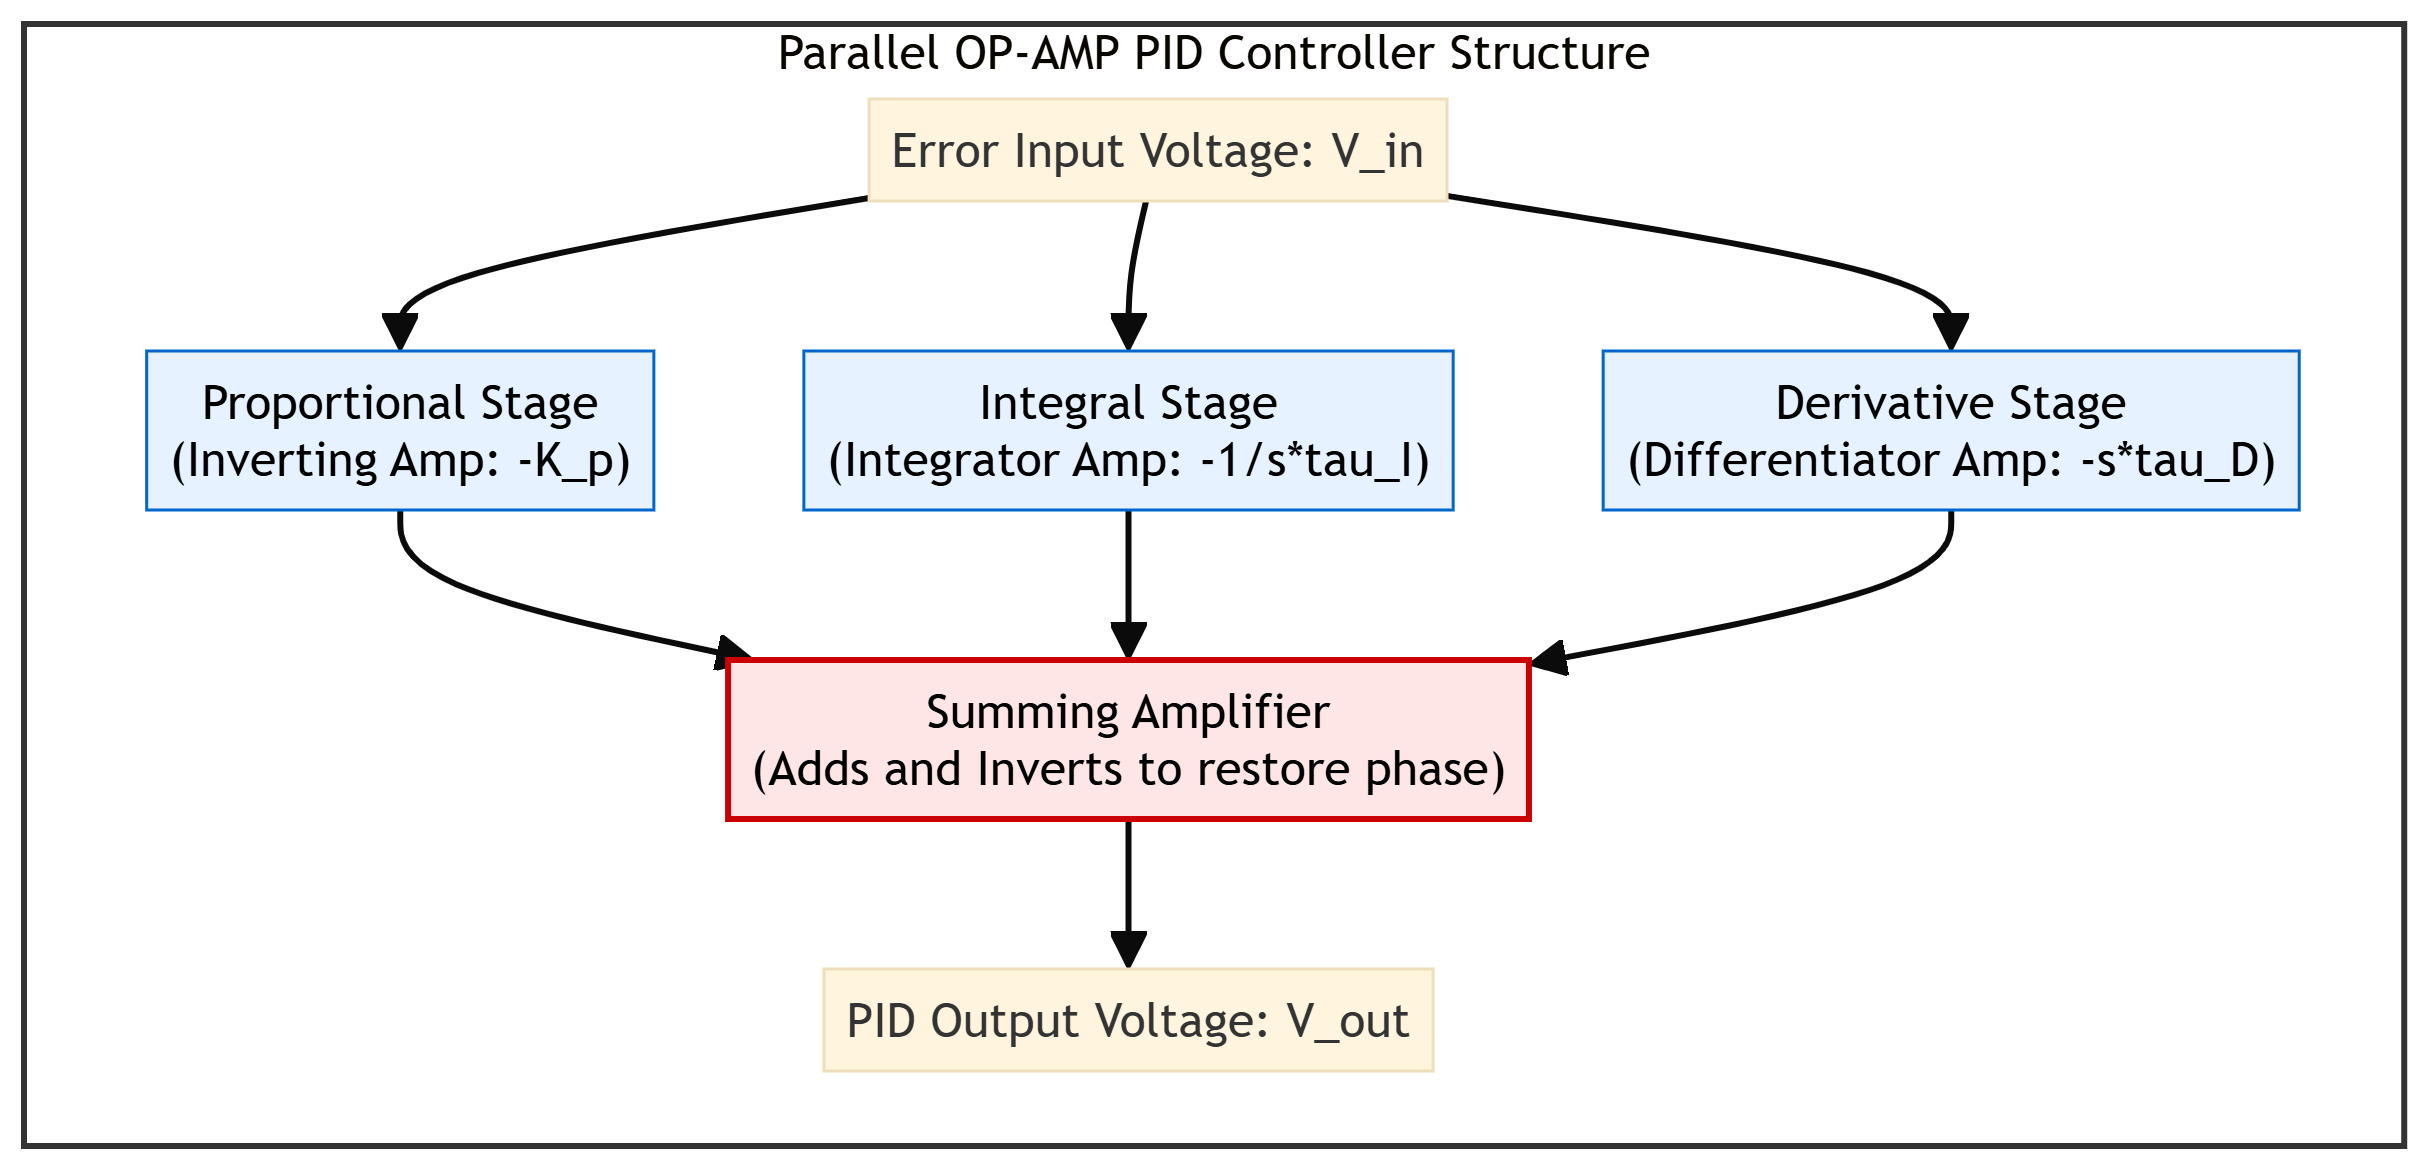
\includegraphics[width=0.75\textwidth,height=0.32\textheight,keepaspectratio]{../Images/chapter_02/opamp_pid_parallel.png}
\caption{Parallel OP-AMP PID Controller}
\end{figure}

\subsection{8. PLC Architecture (Unit III)}
Internal modules showing CPU, memory, power supply, system bus, and input/output interface cards.
\begin{figure}[H]
\centering
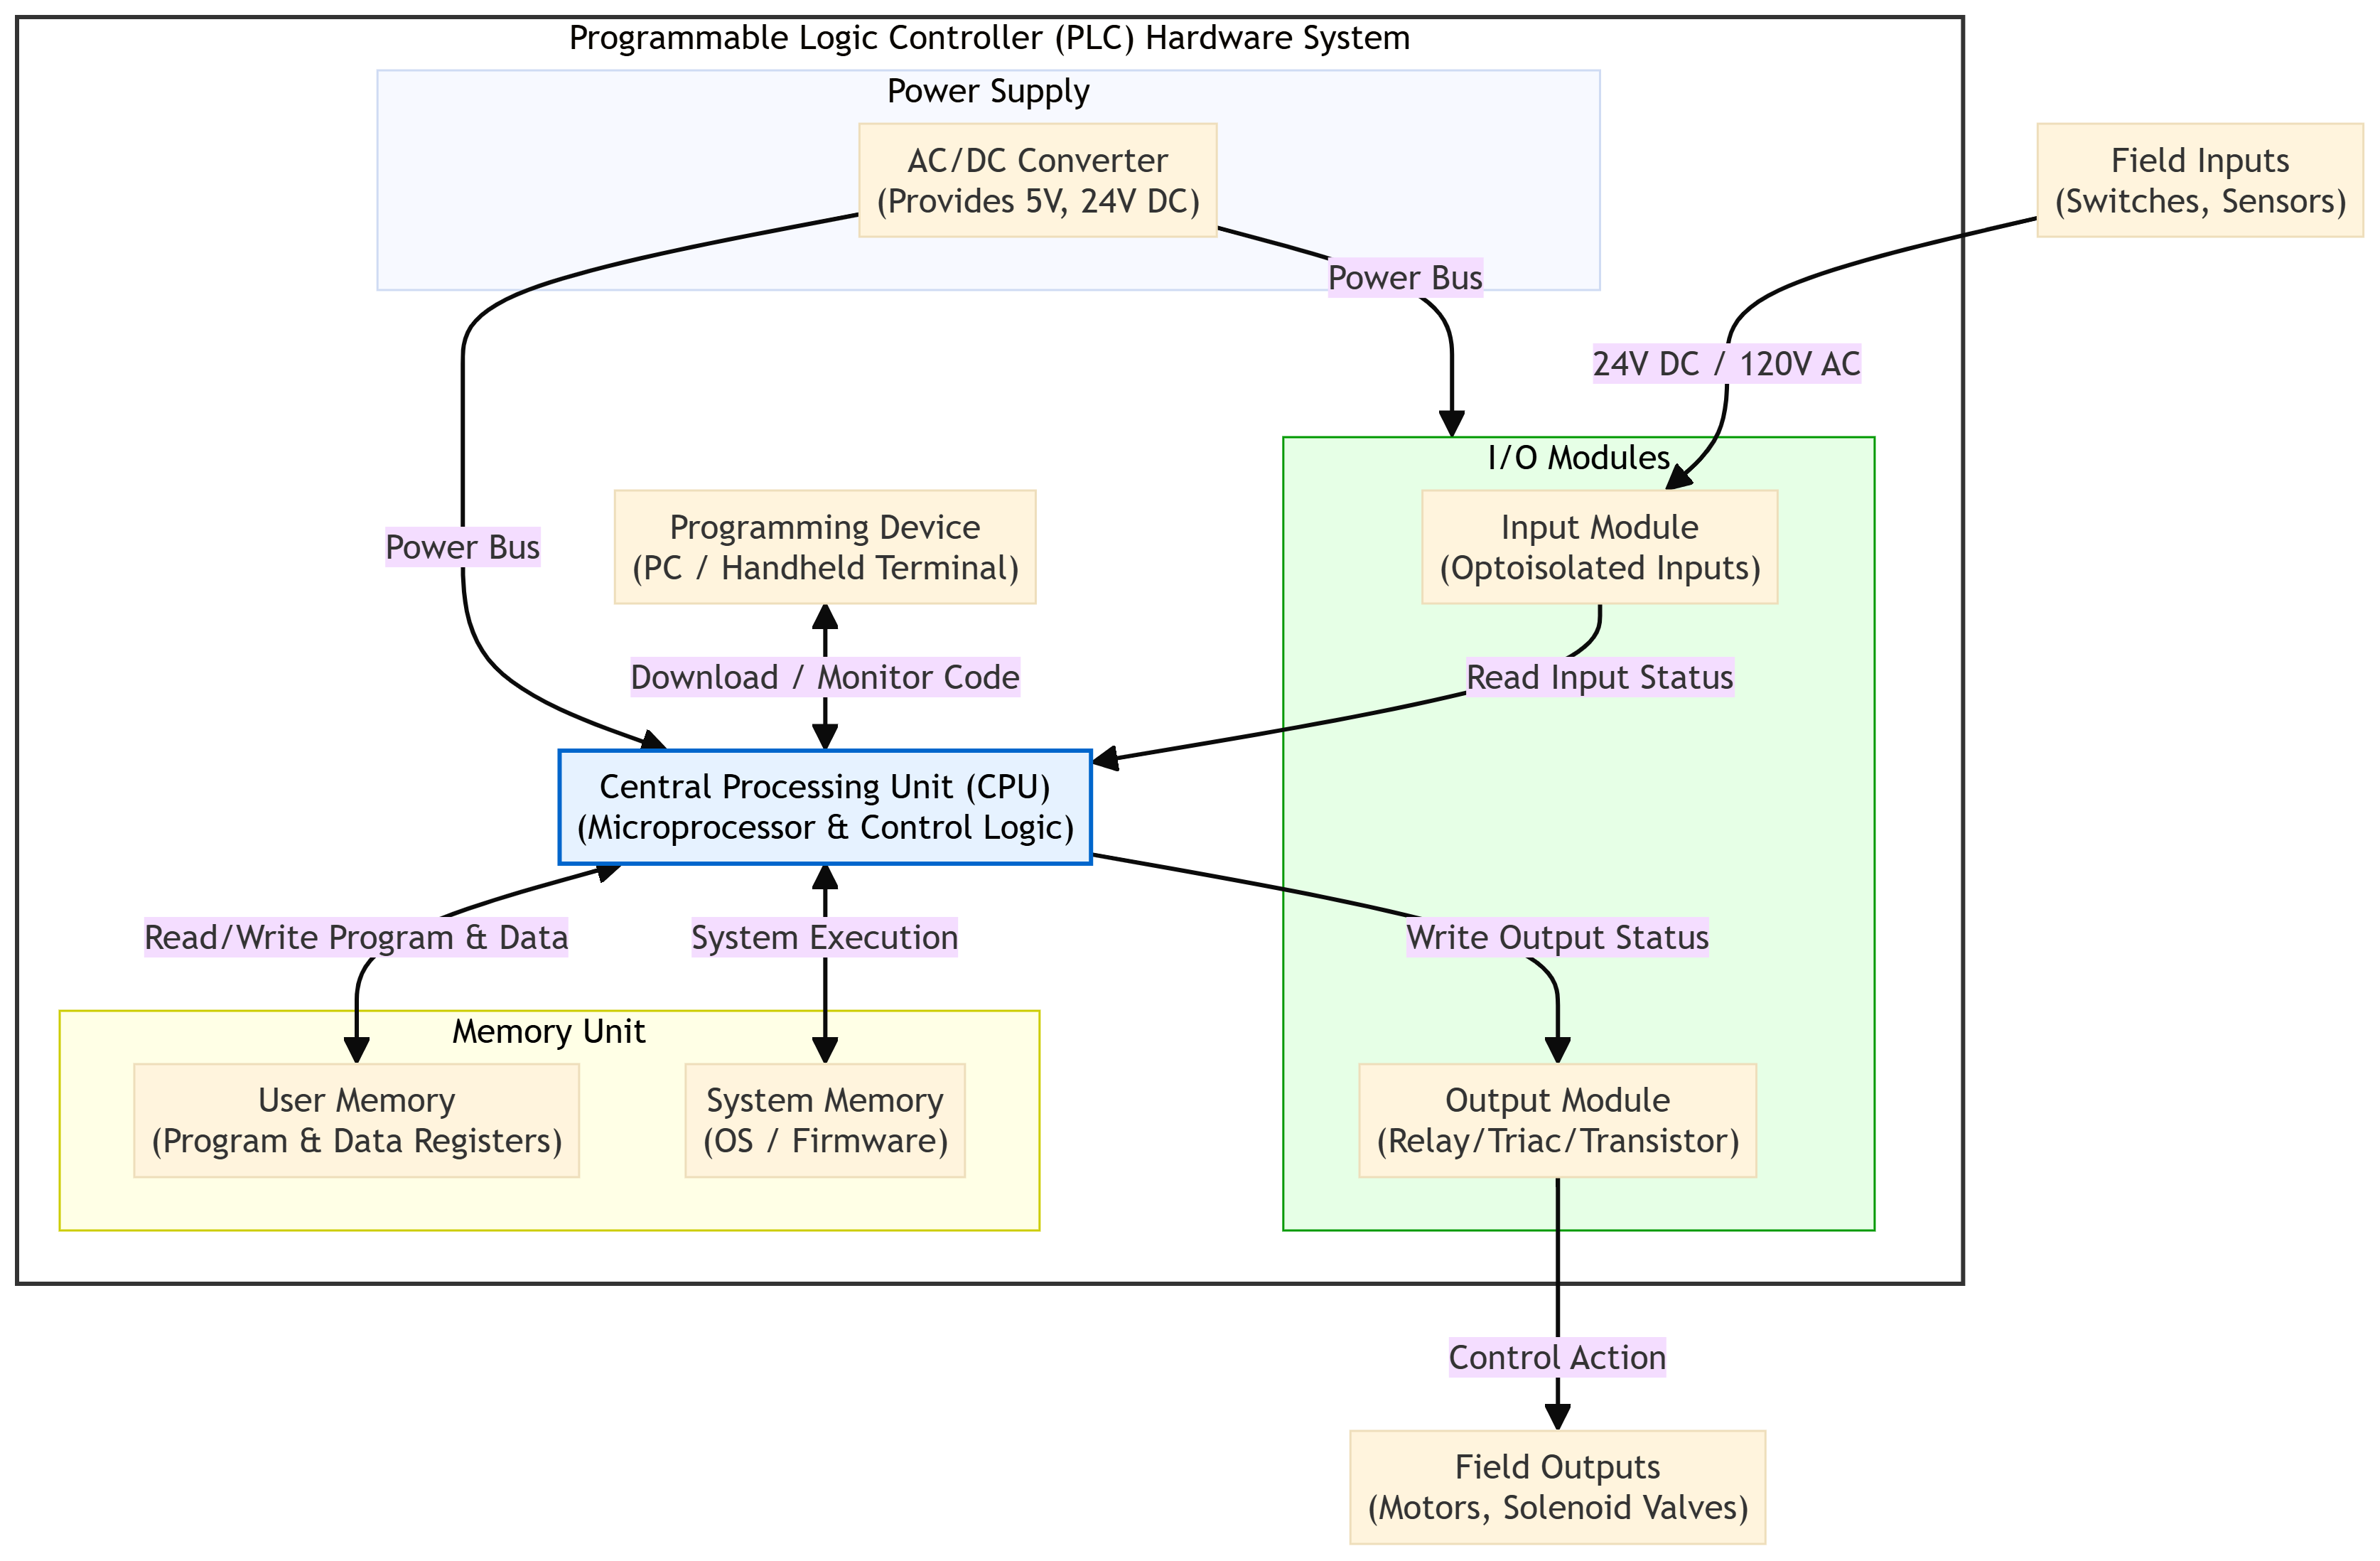
\includegraphics[width=0.75\textwidth,height=0.32\textheight,keepaspectratio]{../Images/chapter_03/plc_architecture.png}
\caption{PLC Hardware Architecture Block Diagram}
\end{figure}

\subsection{9. PLC Ladder Logic (Unit III)}
Start/Stop latch logic and Auto-Filling tank logic.
\begin{figure}[H]
\centering
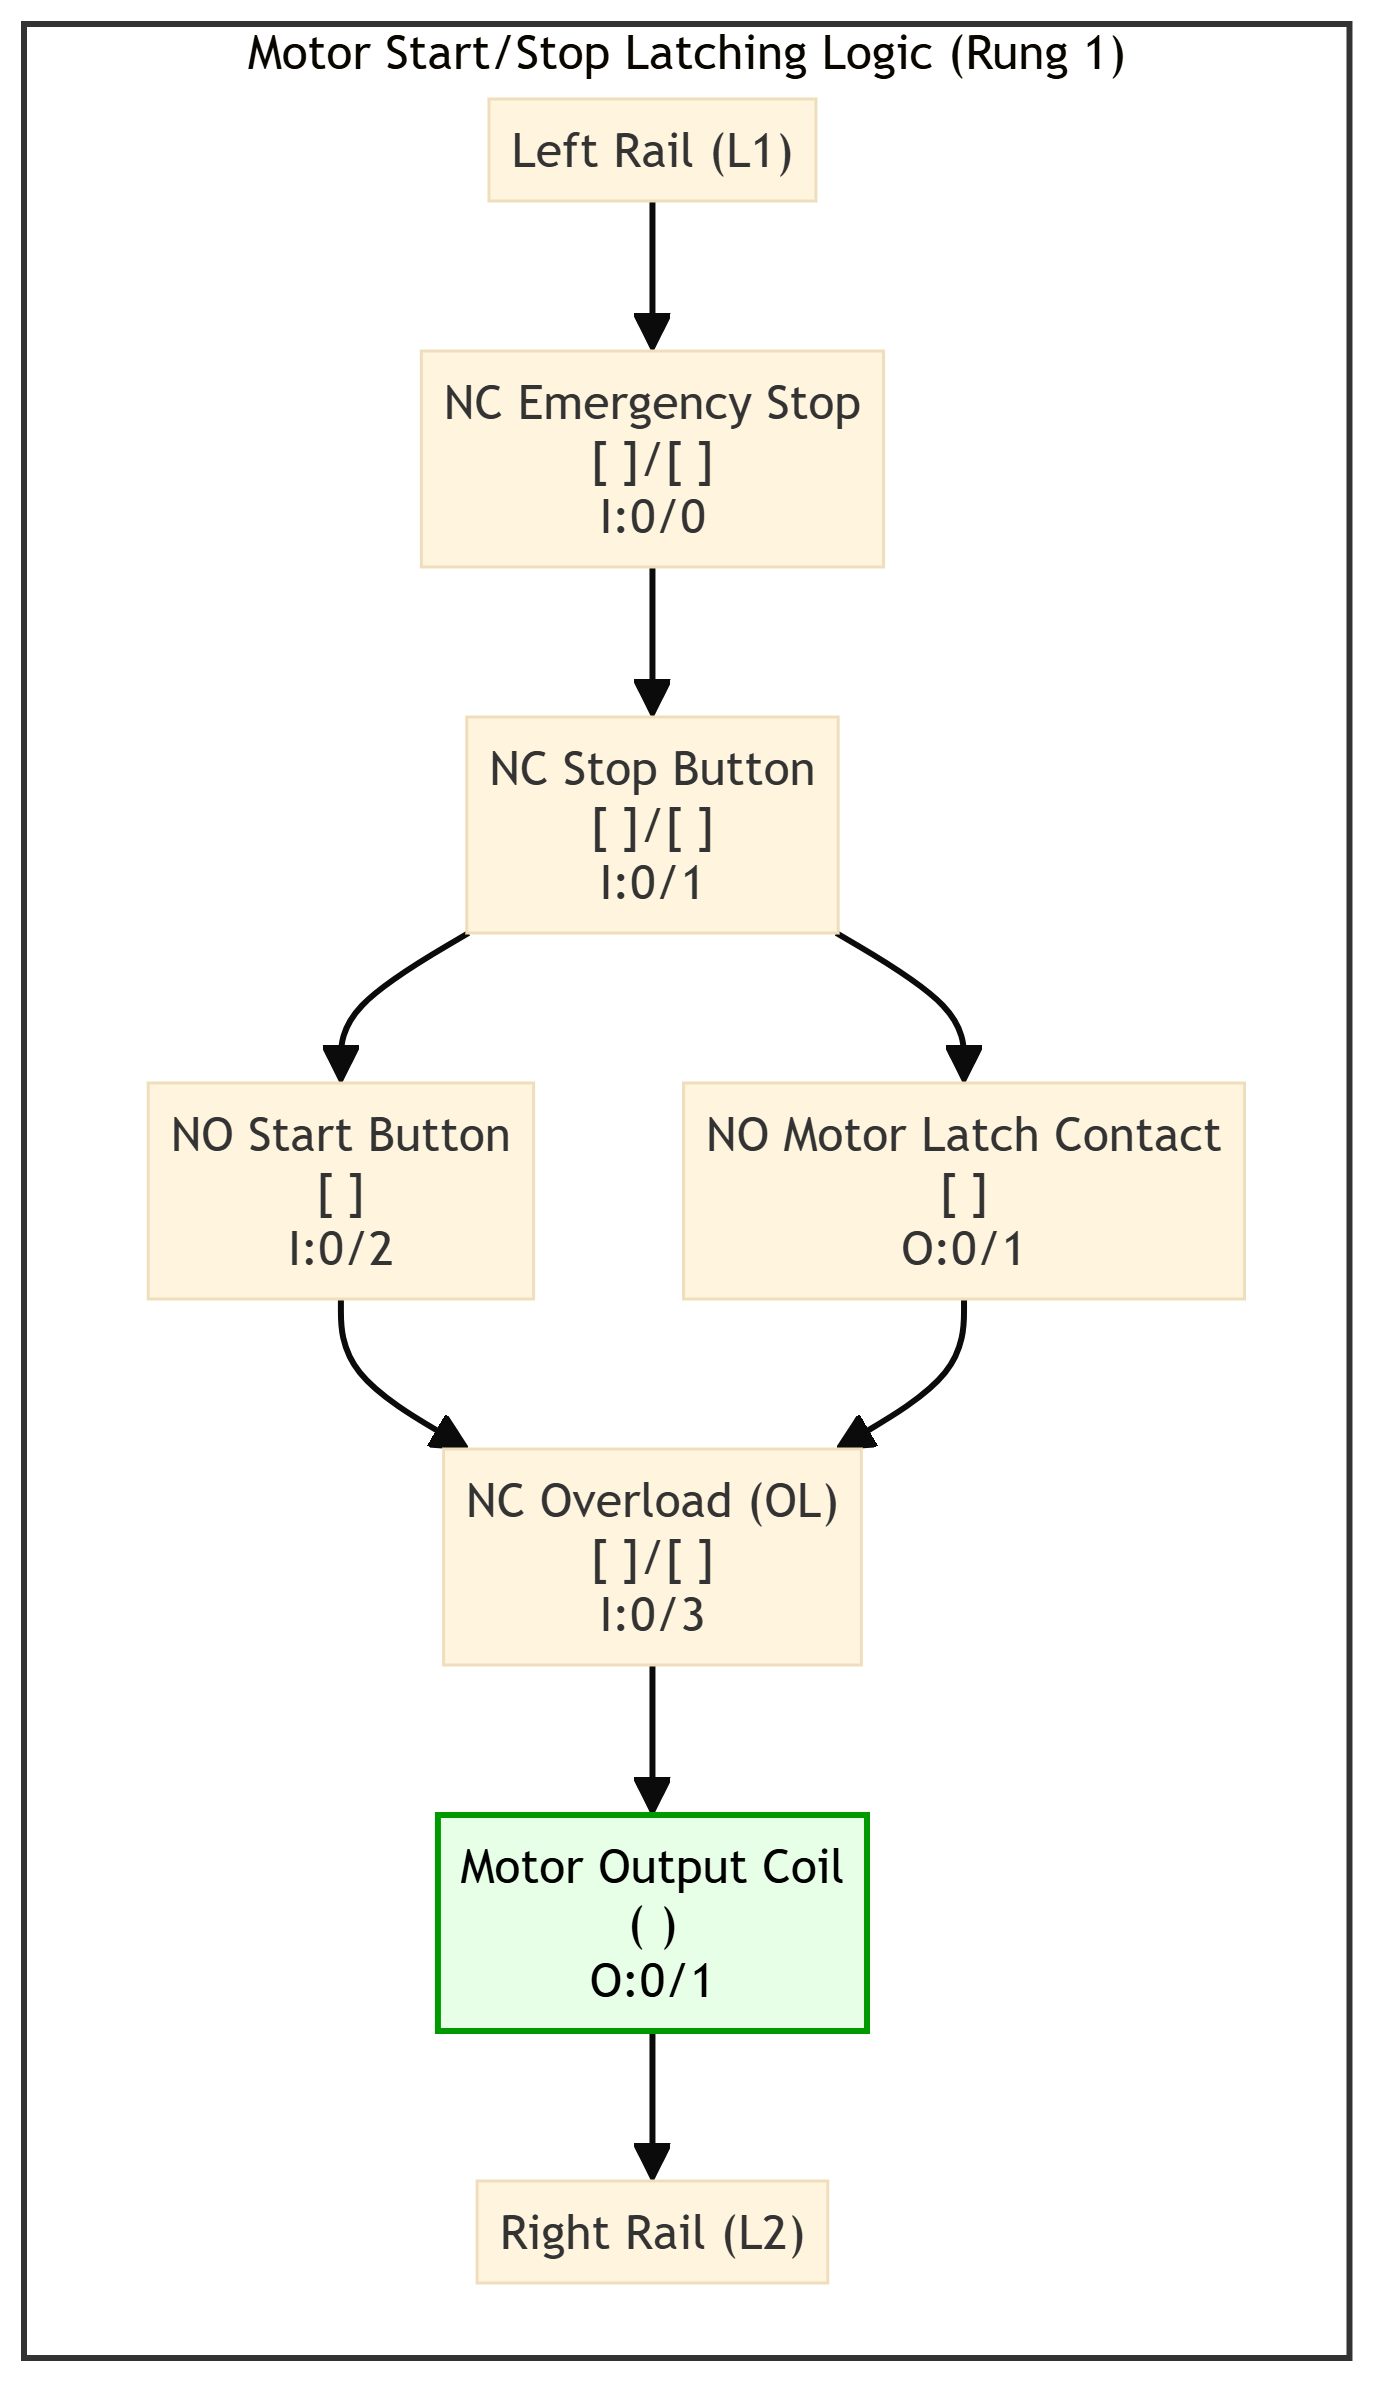
\includegraphics[width=0.75\textwidth,height=0.32\textheight,keepaspectratio]{../Images/chapter_03/motor_latch.png}
\caption{Motor Start/Stop Latching Control}
\end{figure}
\begin{figure}[H]
\centering
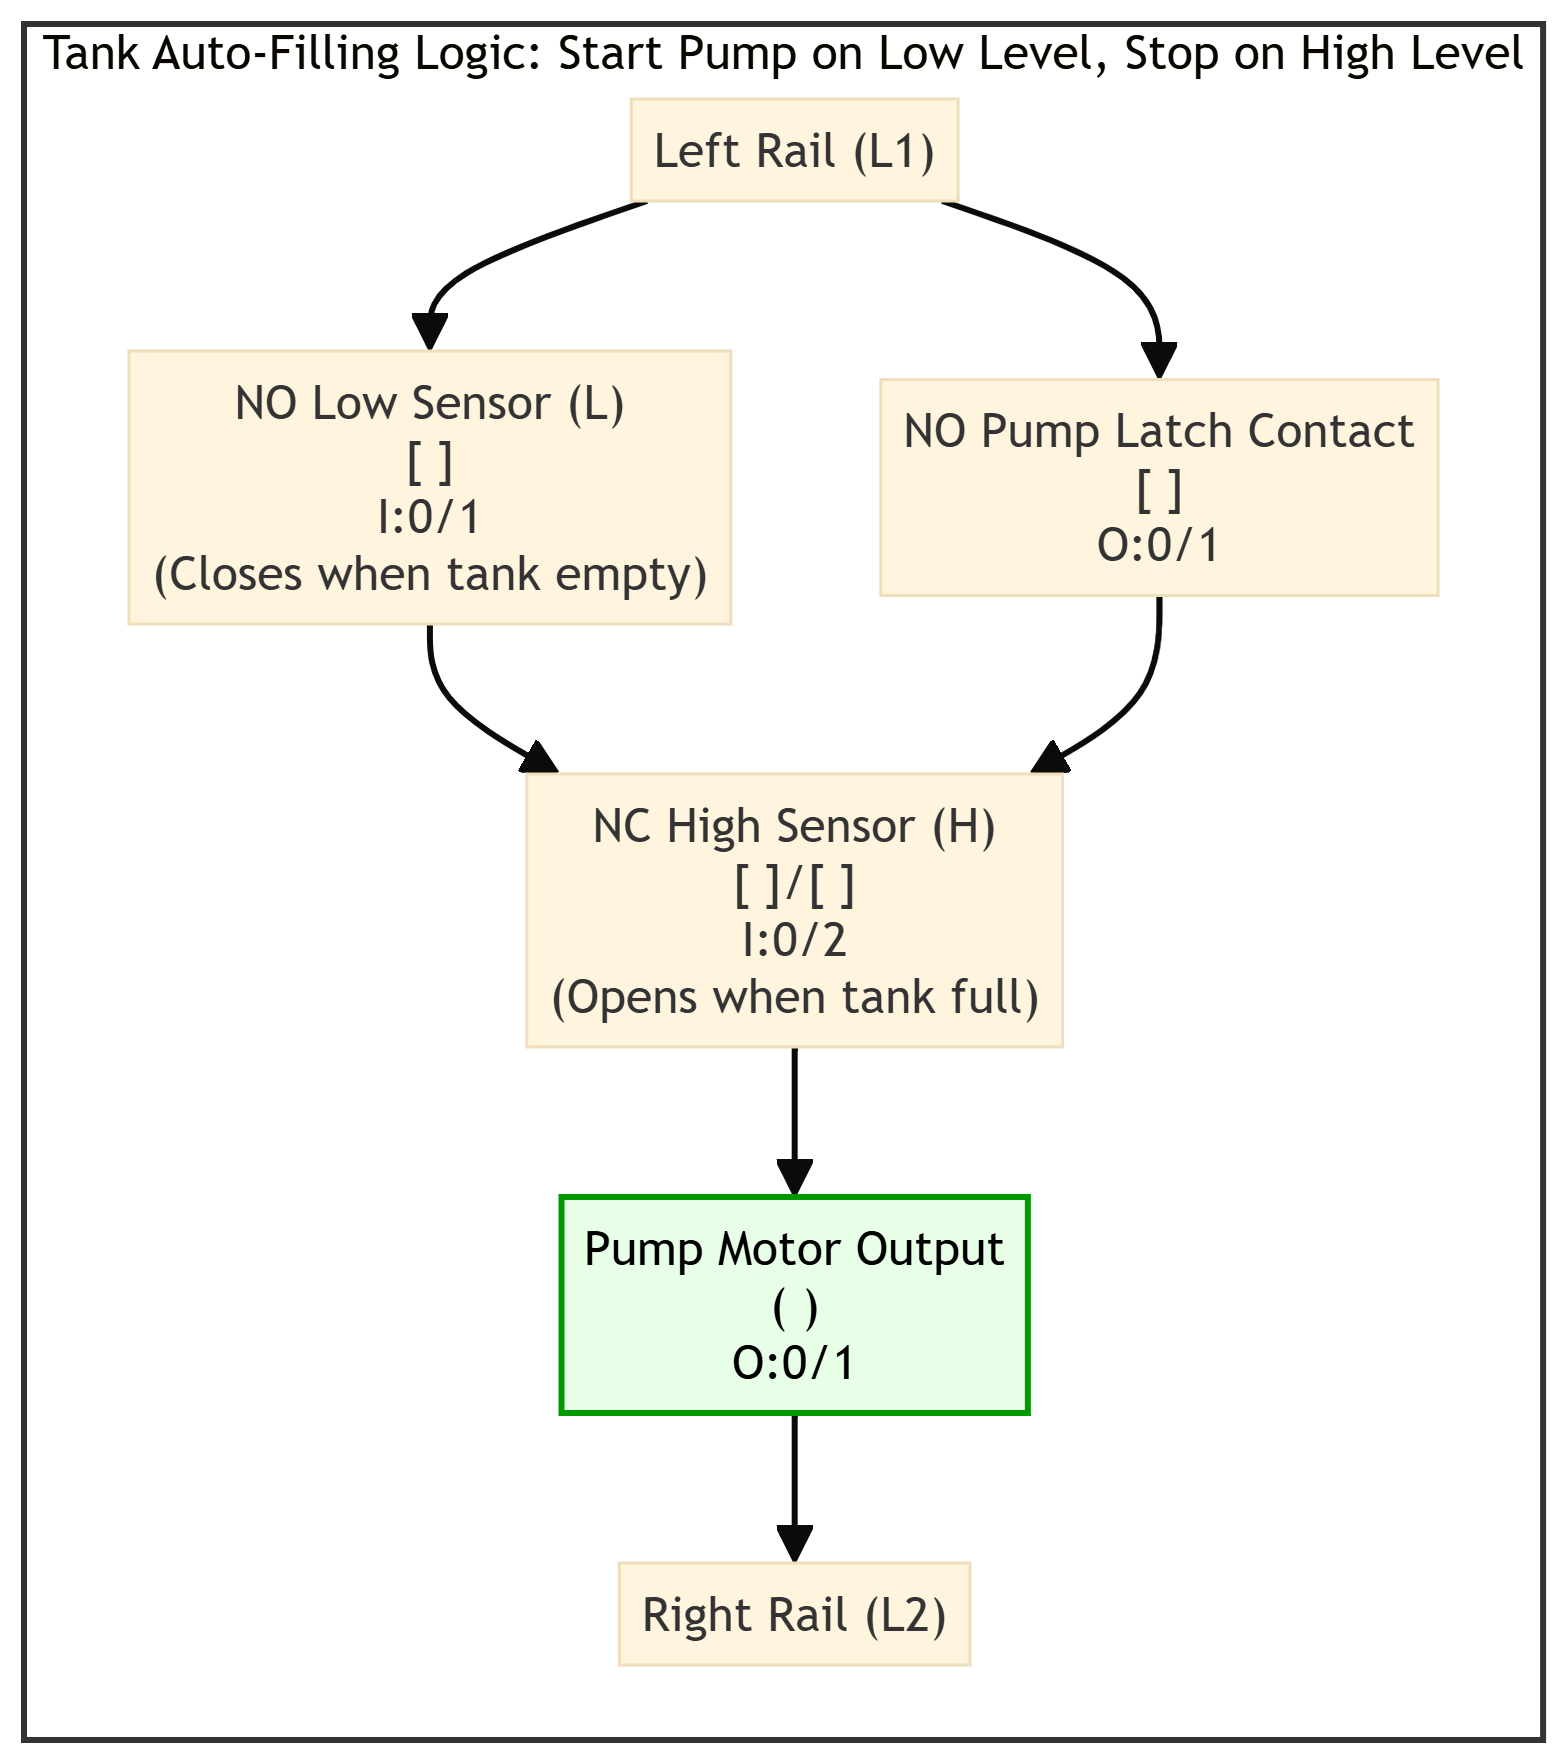
\includegraphics[width=0.75\textwidth,height=0.32\textheight,keepaspectratio]{../Images/chapter_03/tank_level_ladder.png}
\caption{PLC Tank Level Control System}
\end{figure}

\subsection{10. DCS Levels (Unit III)}
The five levels of hierarchical control: Level 0 (Field), Level 1 (Direct Control), Level 2 (Supervisory), Level 3 (Production), and Level 4 (Enterprise).
\begin{figure}[H]
\centering
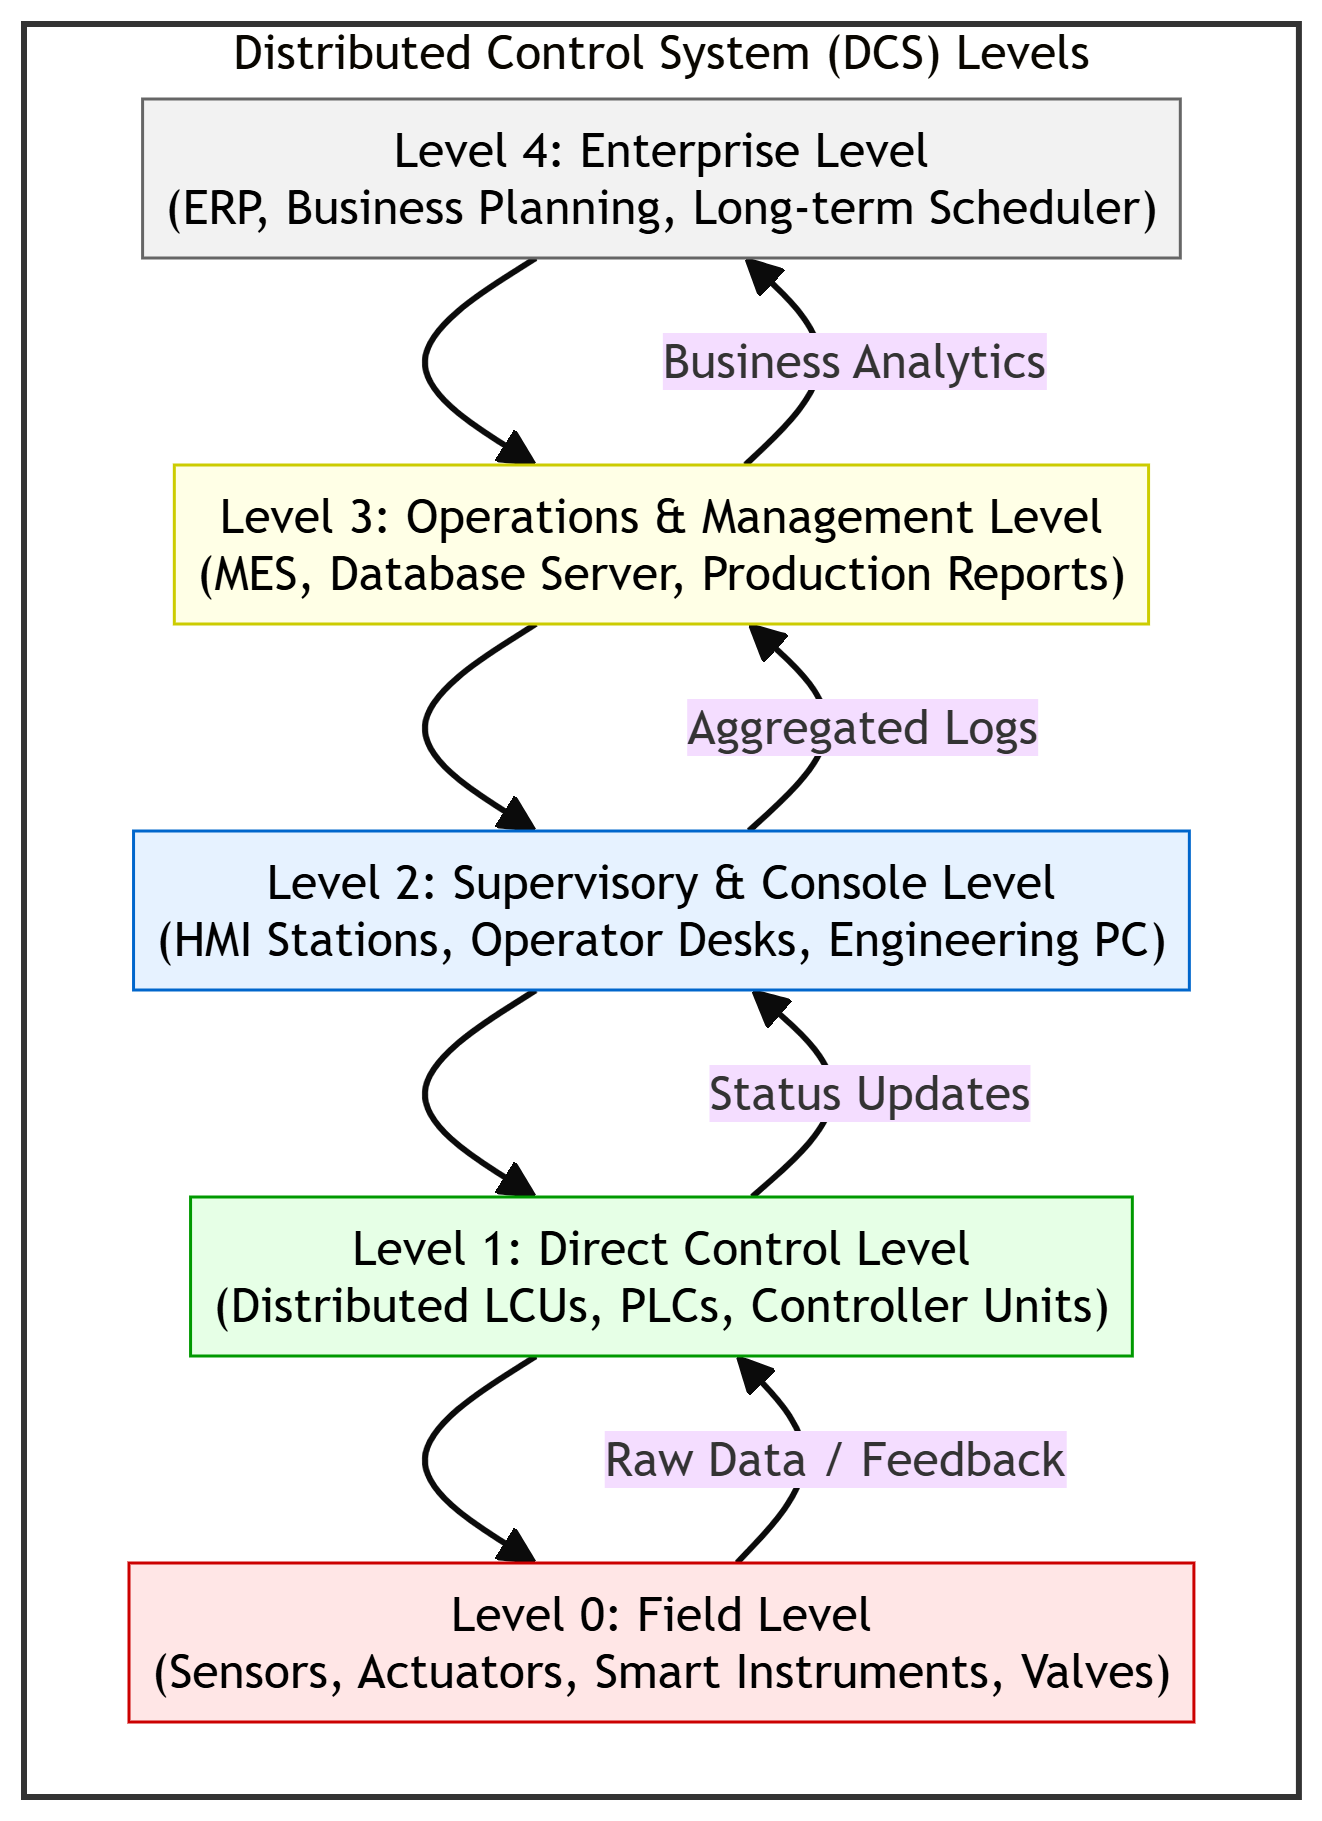
\includegraphics[width=0.75\textwidth,height=0.32\textheight,keepaspectratio]{../Images/chapter_03/dcs_hierarchy.png}
\caption{DCS Hierarchical Levels}
\end{figure}

\subsection{11. SCADA Structure (Unit III)}
Geographically distributed control architecture showing the Master Terminal Unit (MTU), Remote Terminal Units (RTUs), PLCs, and WAN link.
\begin{figure}[H]
\centering
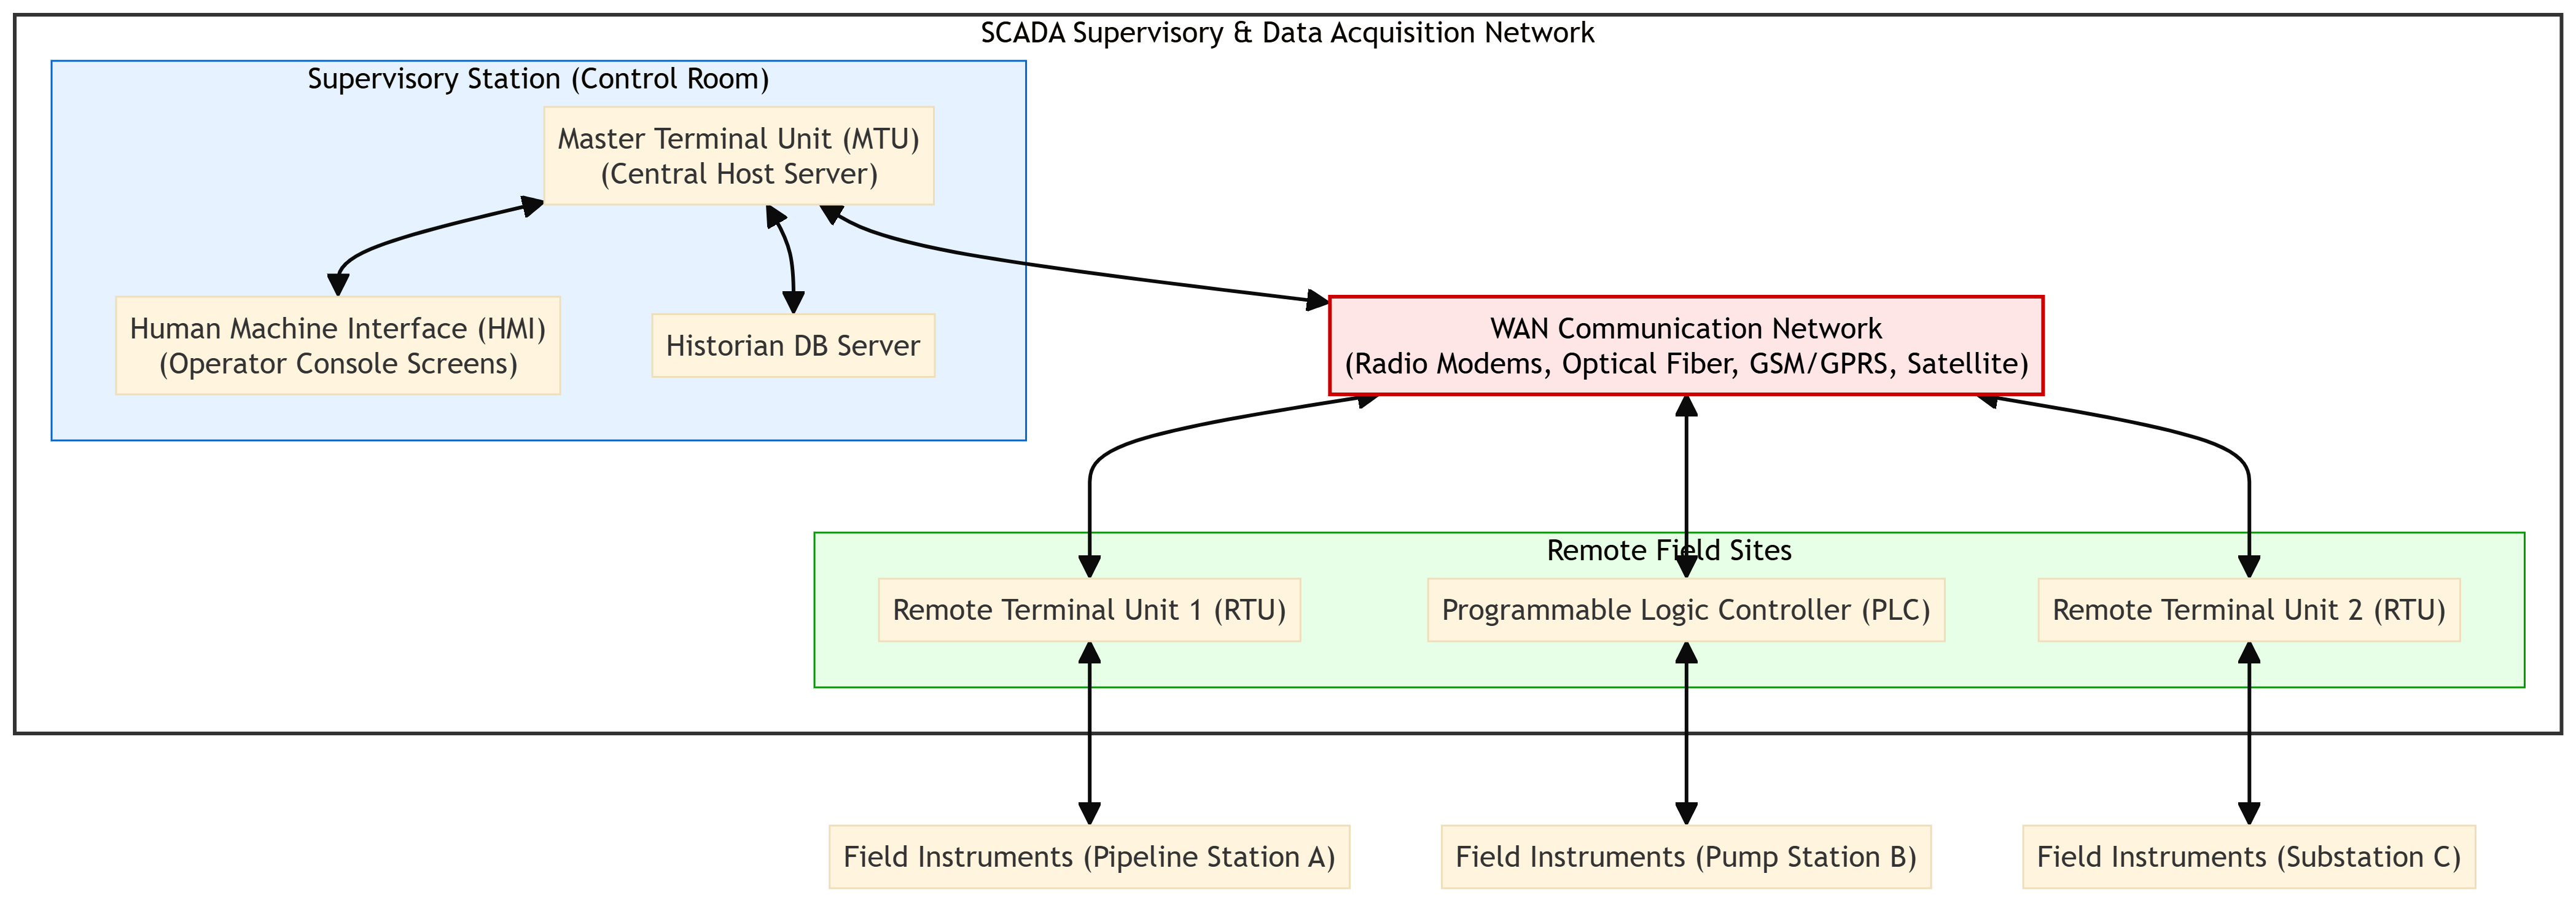
\includegraphics[width=0.75\textwidth,height=0.32\textheight,keepaspectratio]{../Images/chapter_03/scada_architecture.png}
\caption{SCADA System Topology Block Diagram}
\end{figure}

\subsection{12. Cascade Control Loop (Unit IV)}
Nested block diagram featuring a primary (outer) loop controller and a fast secondary (inner) loop controller.
\begin{figure}[H]
\centering
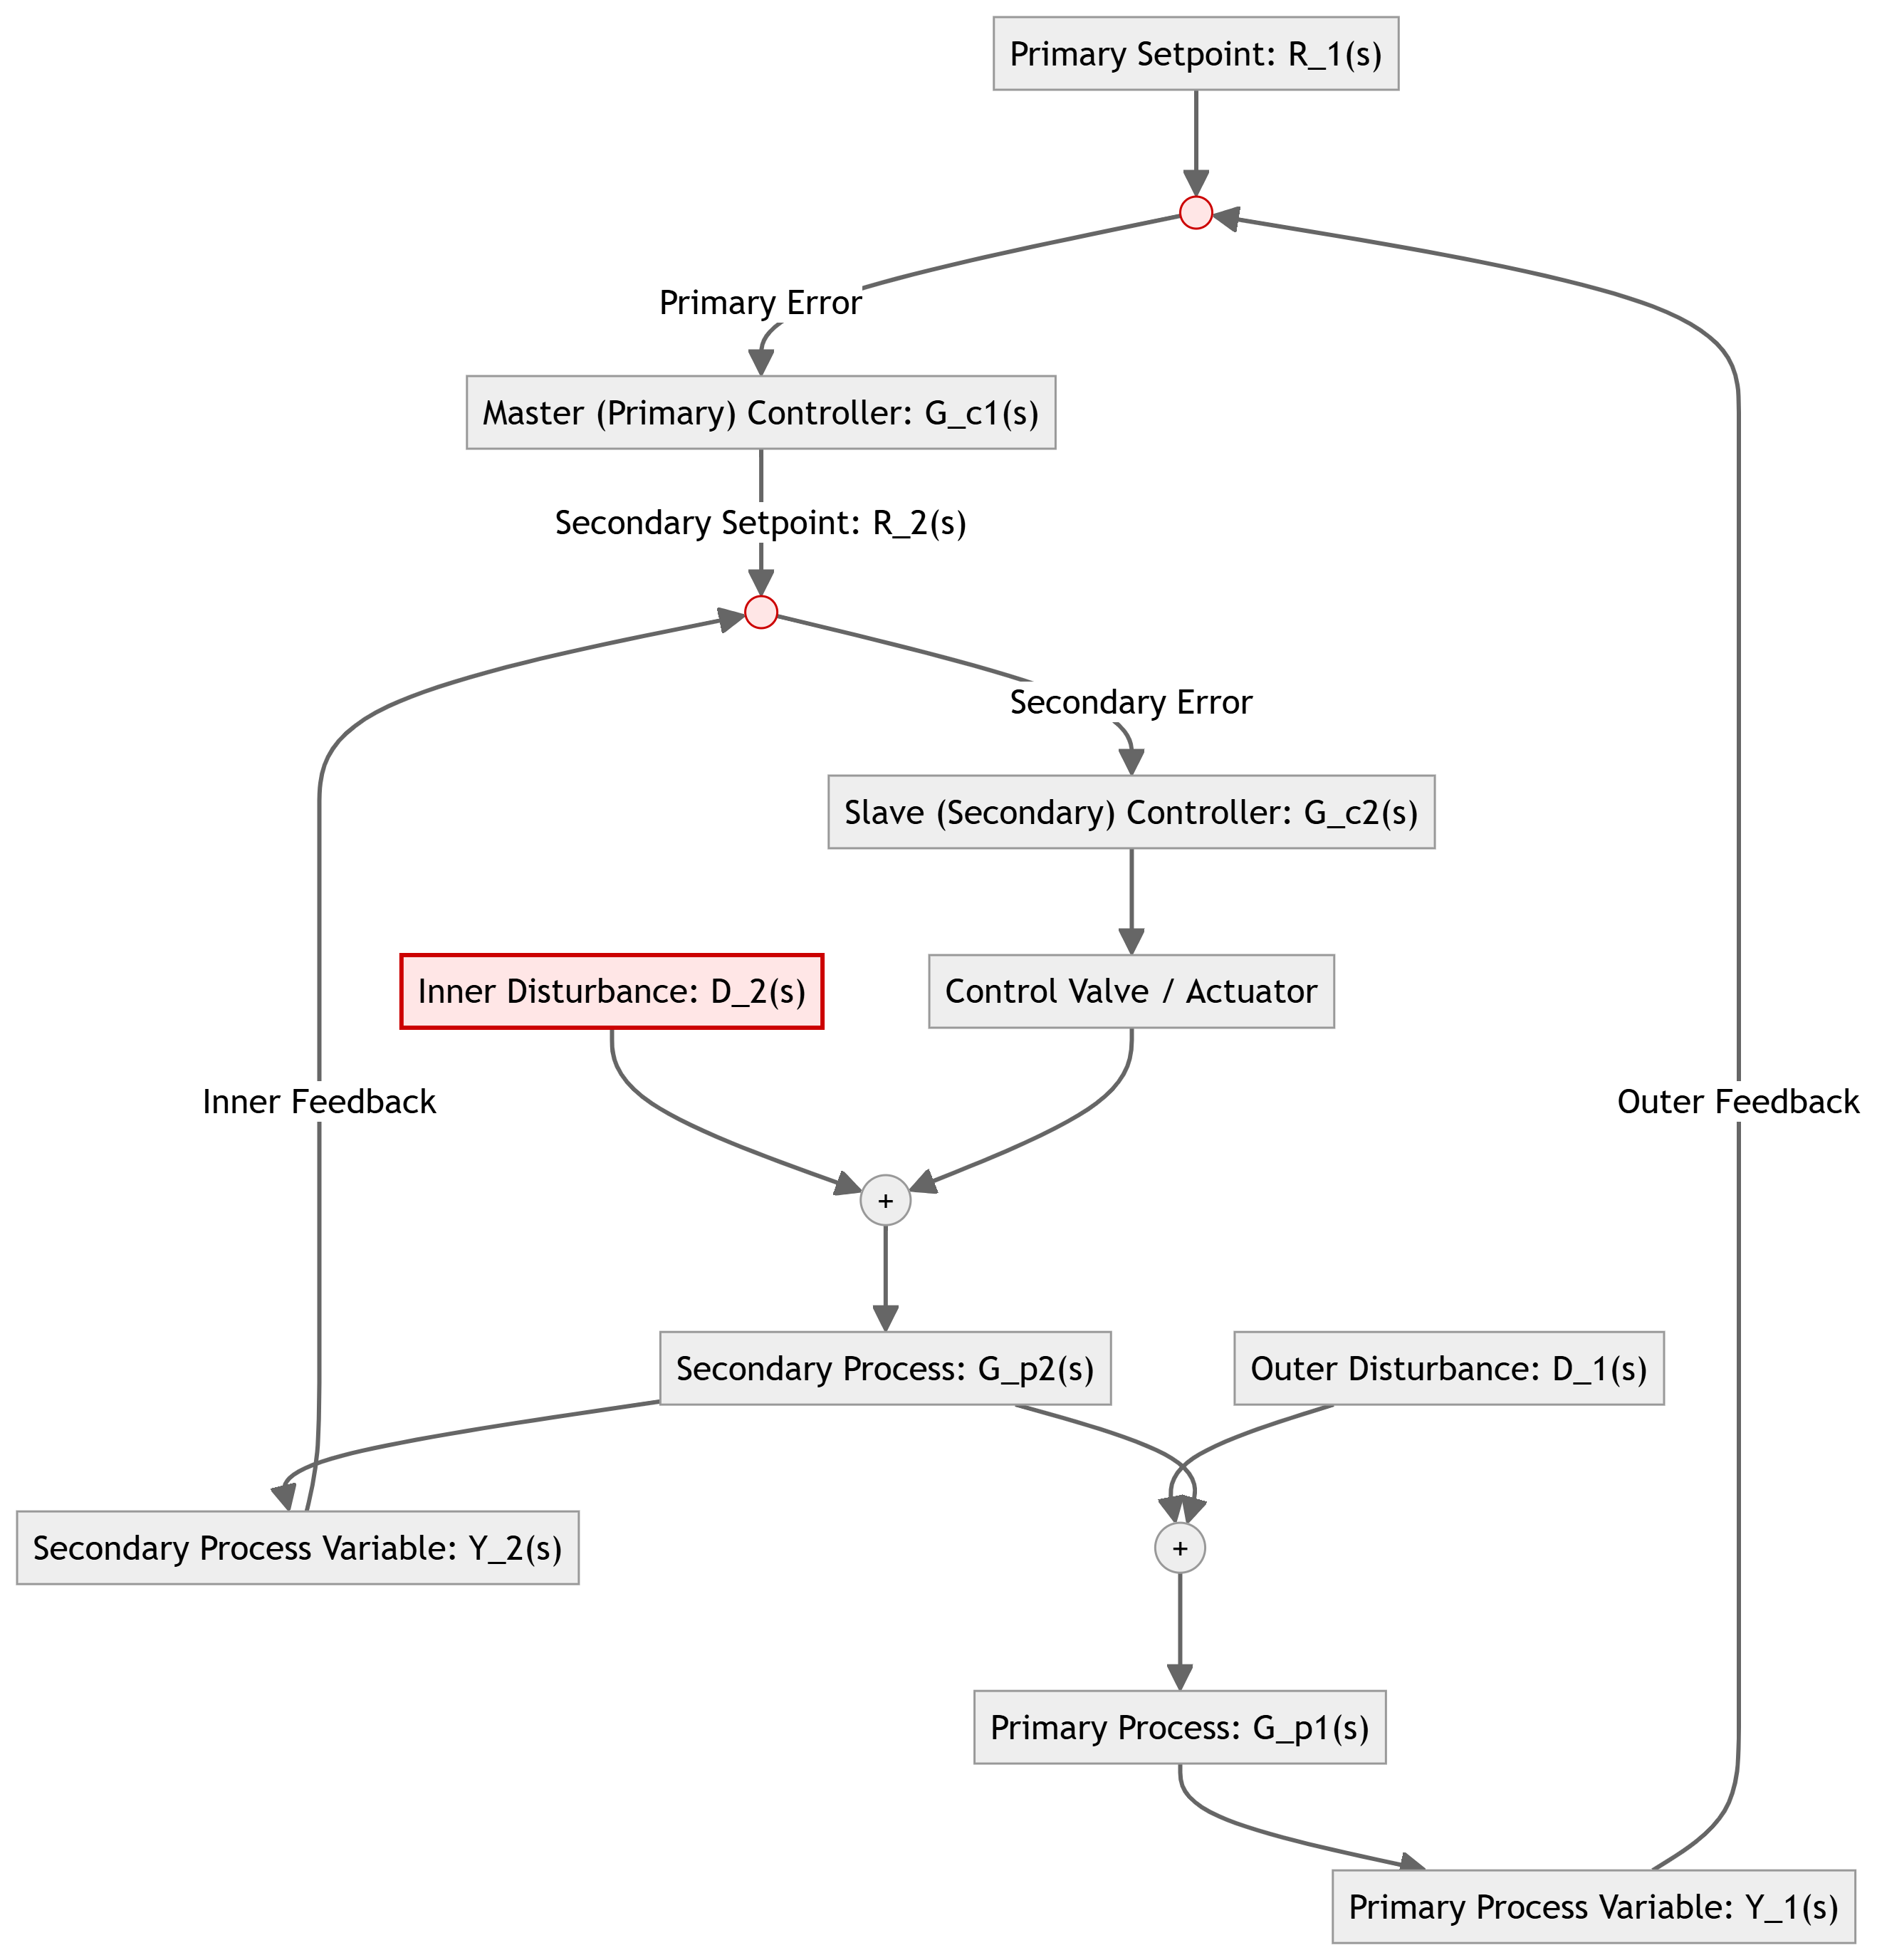
\includegraphics[width=0.75\textwidth,height=0.32\textheight,keepaspectratio]{../Images/chapter_04/cascade_block.png}
\caption{Cascade Control Loop Block Diagram}
\end{figure}

\subsection{13. Override Control (Unit IV)}
Selective control block diagram implementing high/low limit selection to protect hardware.
\begin{figure}[H]
\centering
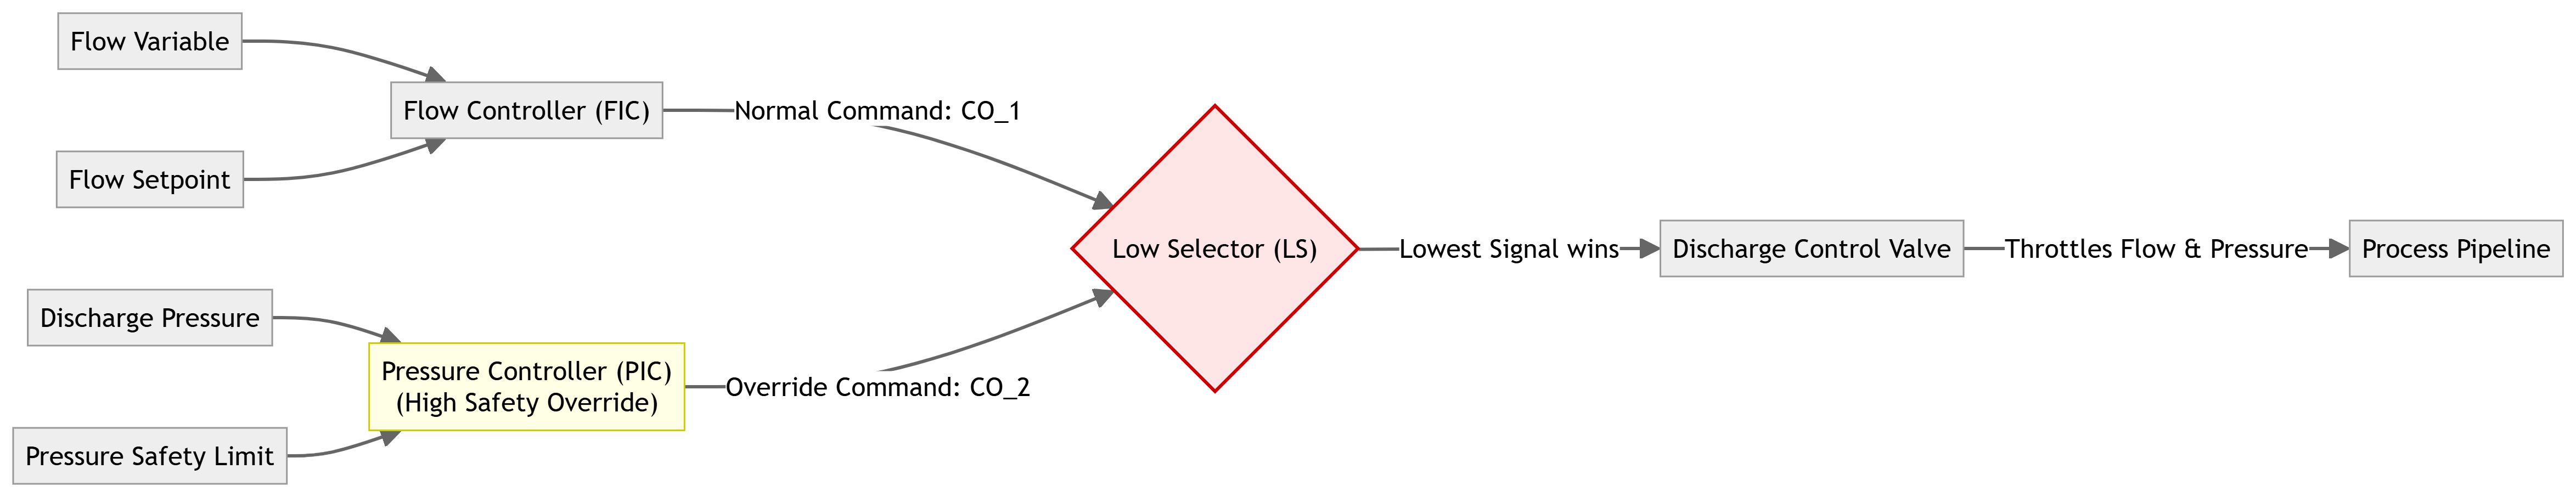
\includegraphics[width=0.75\textwidth,height=0.32\textheight,keepaspectratio]{../Images/chapter_04/override_control.png}
\caption{Override (Selective) Control Loop}
\end{figure}

\subsection{14. Split-Range Control (Unit IV)}
Response curves demonstrating a single controller command split to drive multiple actuators sequentially.
\begin{figure}[H]
\centering
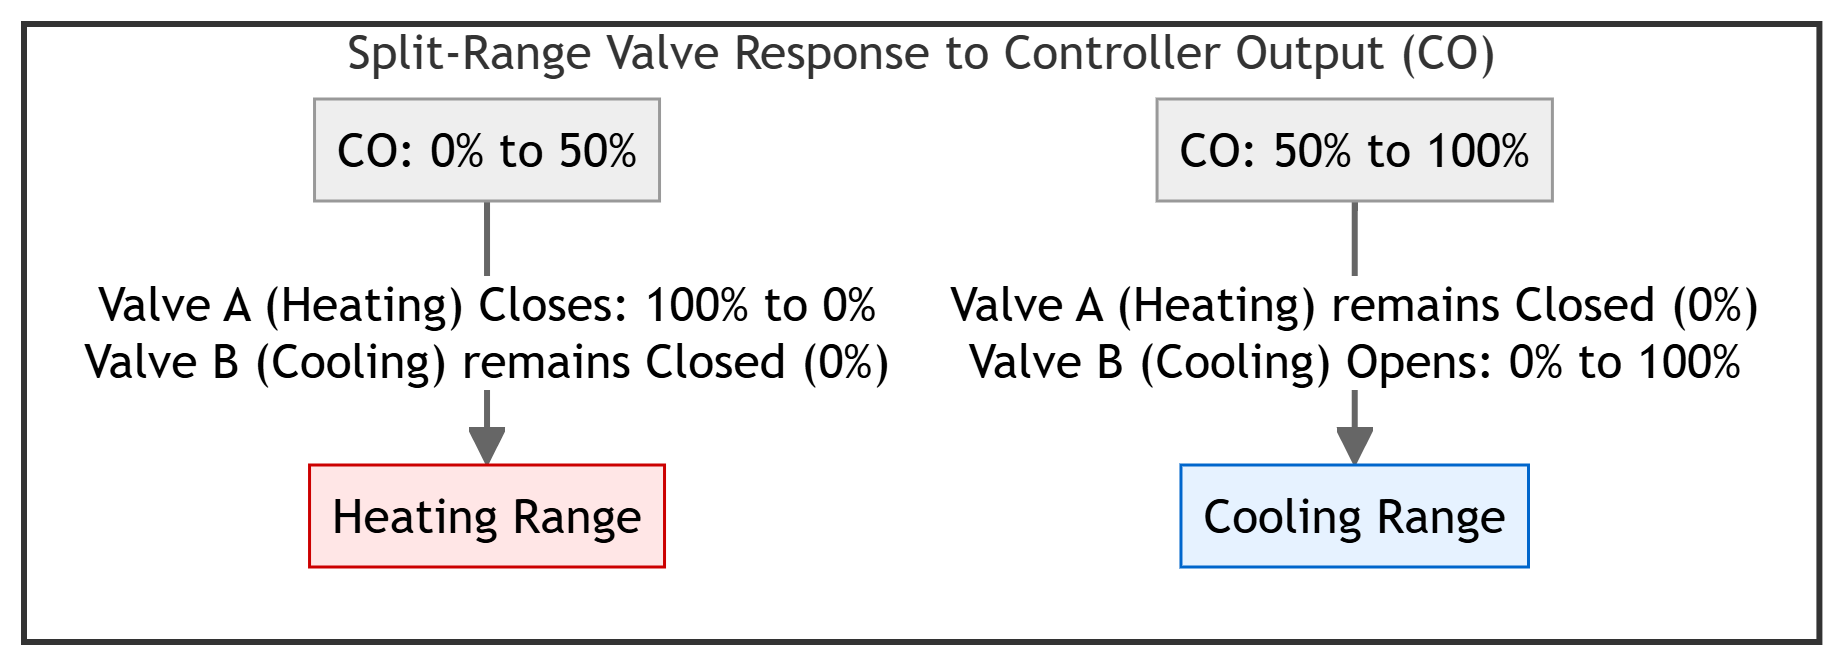
\includegraphics[width=0.75\textwidth,height=0.32\textheight,keepaspectratio]{../Images/chapter_04/split_range.png}
\caption{Split-Range (Duplex) Control Loop Graph}
\end{figure}

\subsection{15. Adaptive Controllers (Unit IV)}
Block diagrams for both Model Reference Adaptive Control (MRAC) and Self-Tuning Regulators (STR).
\begin{figure}[H]
\centering
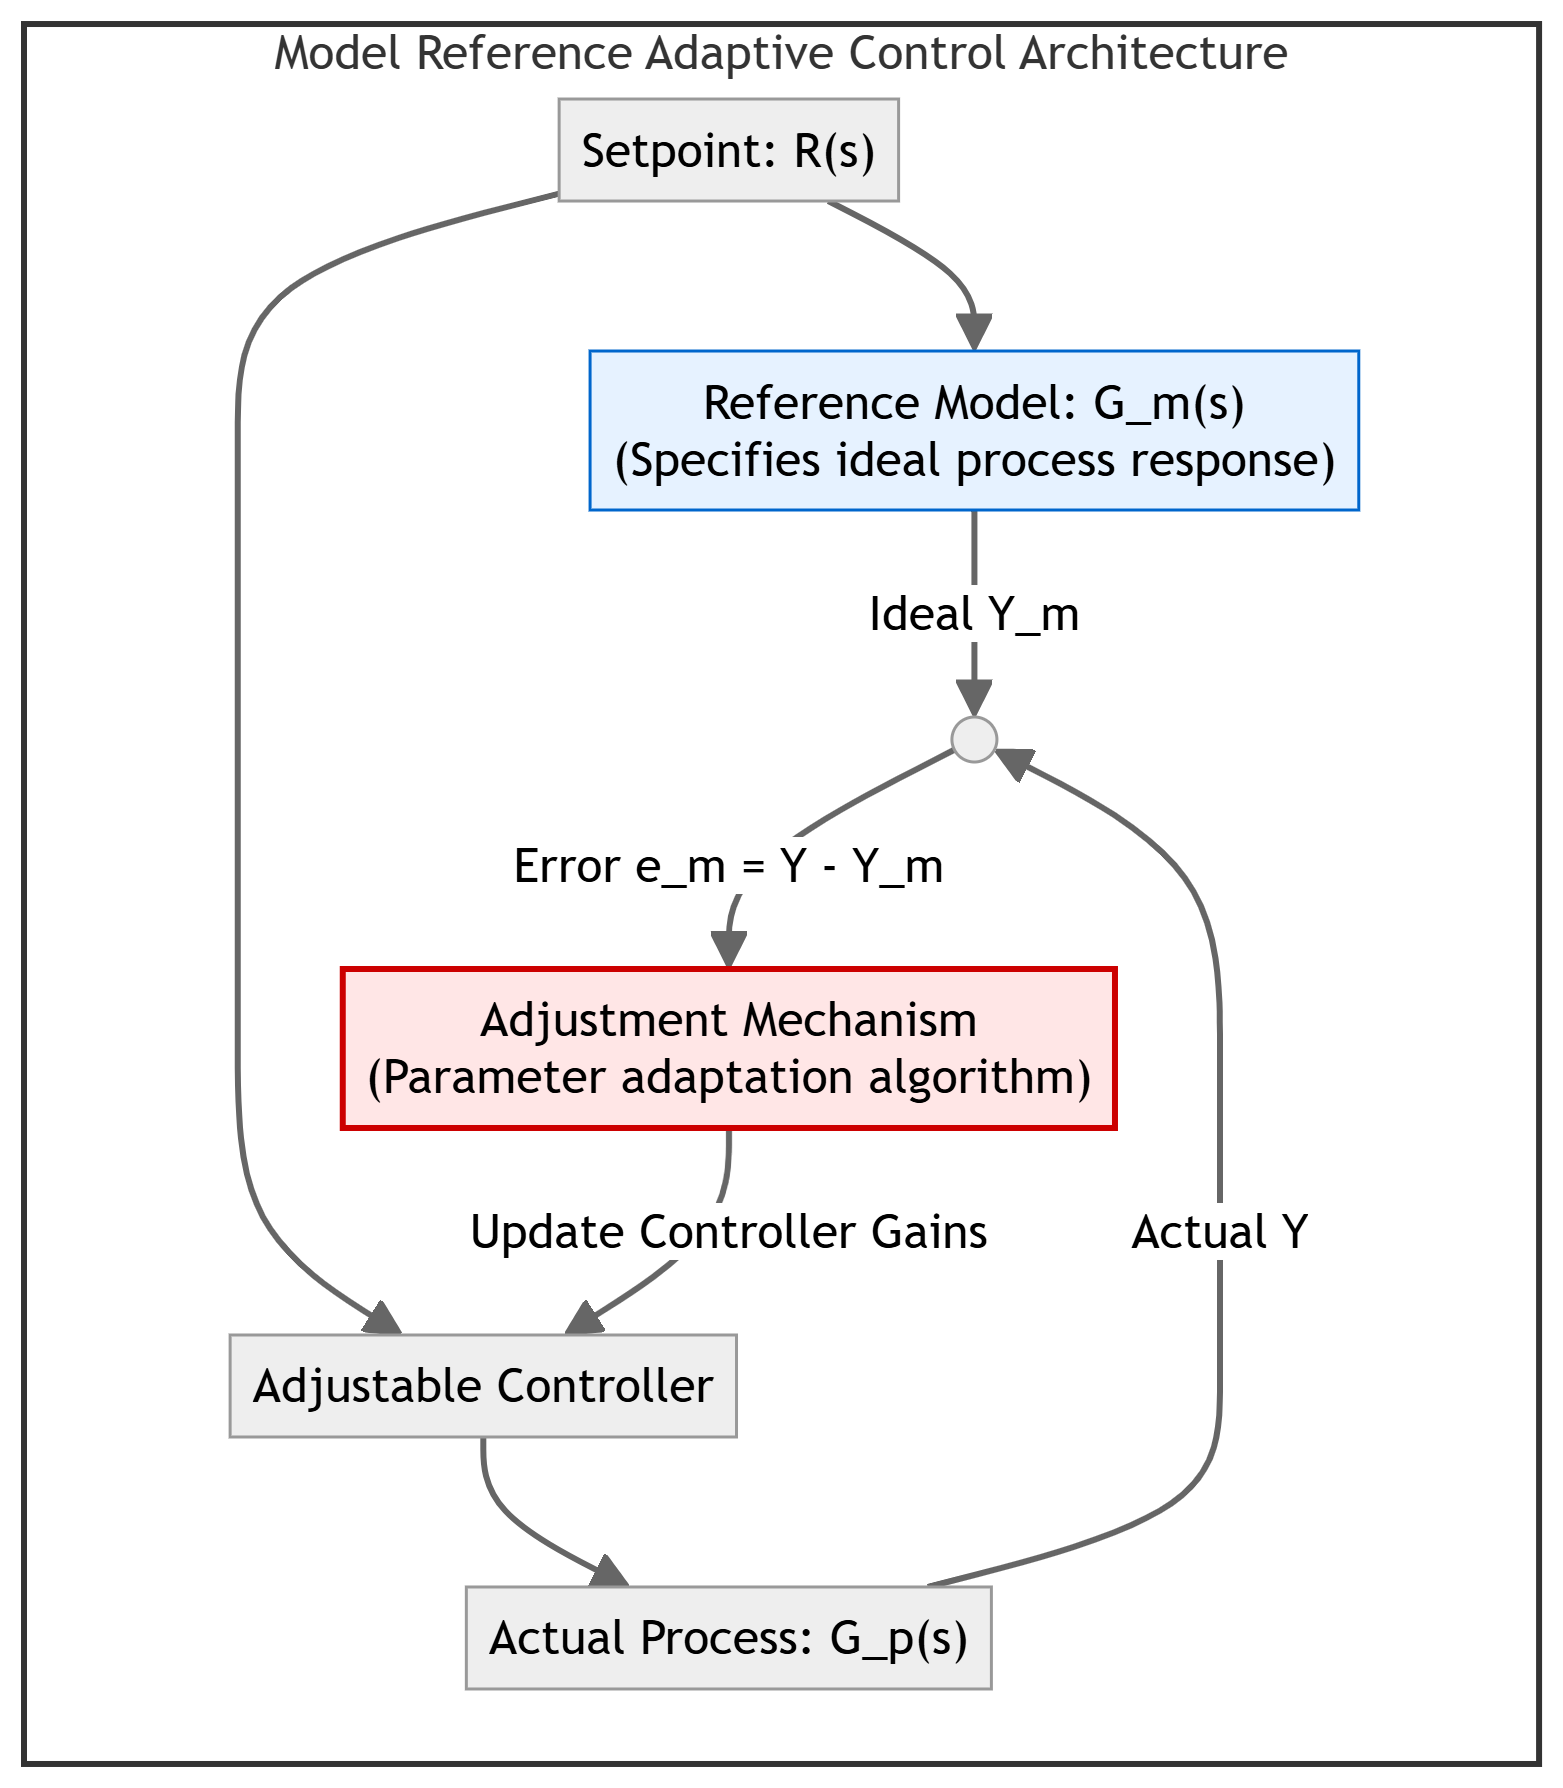
\includegraphics[width=0.75\textwidth,height=0.32\textheight,keepaspectratio]{../Images/chapter_04/mrac_block.png}
\caption{Model Reference Adaptive Control (MRAC)}
\end{figure}
\begin{figure}[H]
\centering
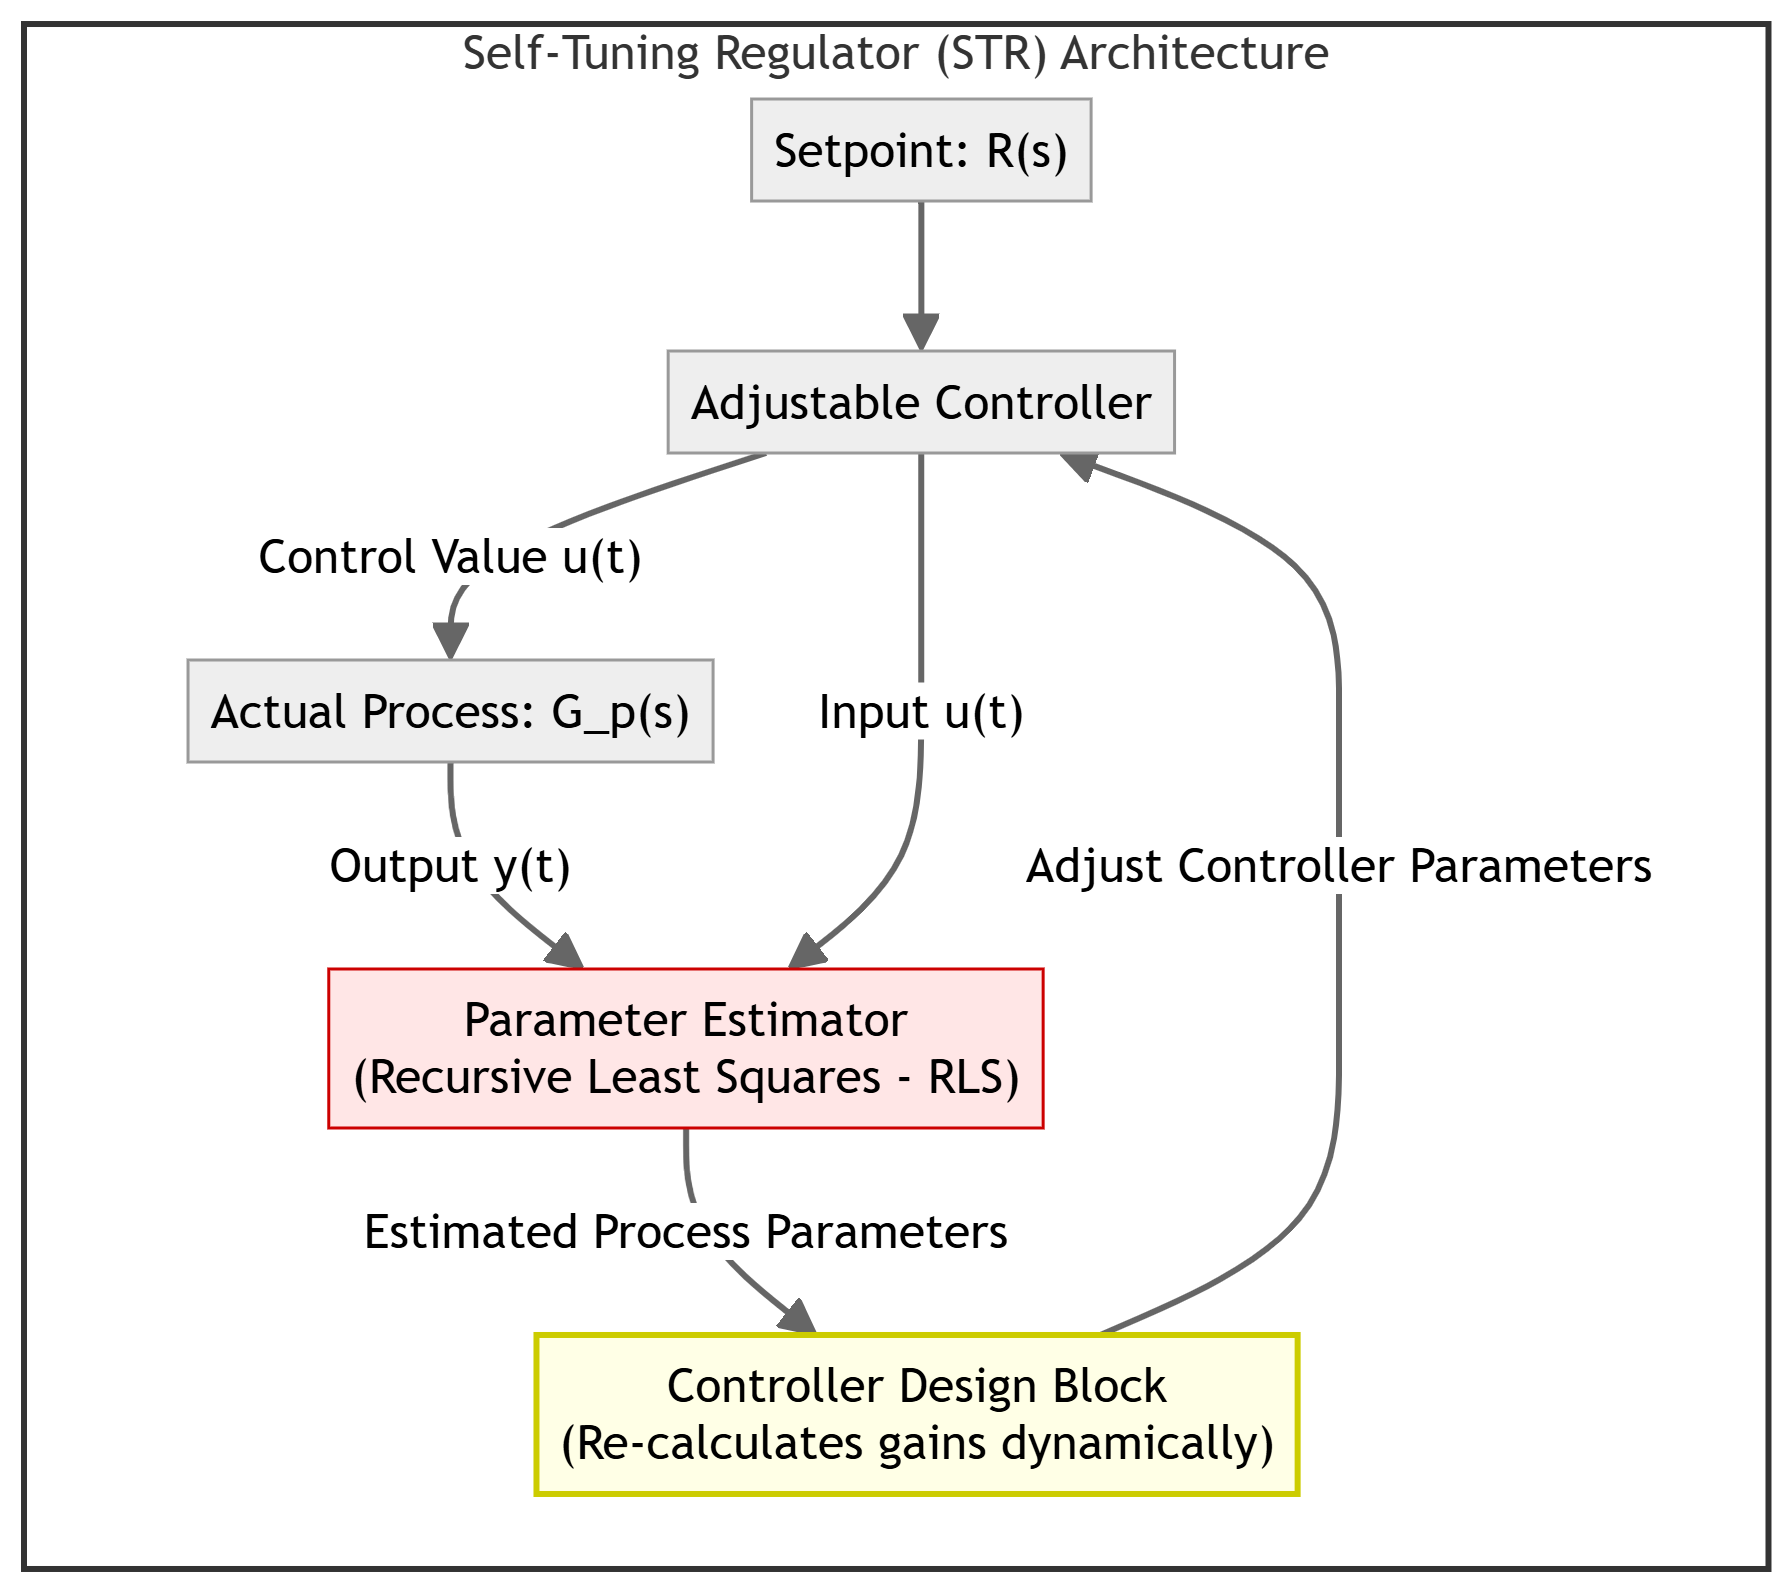
\includegraphics[width=0.75\textwidth,height=0.32\textheight,keepaspectratio]{../Images/chapter_04/str_block.png}
\caption{Self-Tuning Regulator (STR)}
\end{figure}

\subsection{16. IMC Block Diagram (Unit IV)}
Internal Model Control block structure feeding back isolated disturbances to the controller.
\begin{figure}[H]
\centering
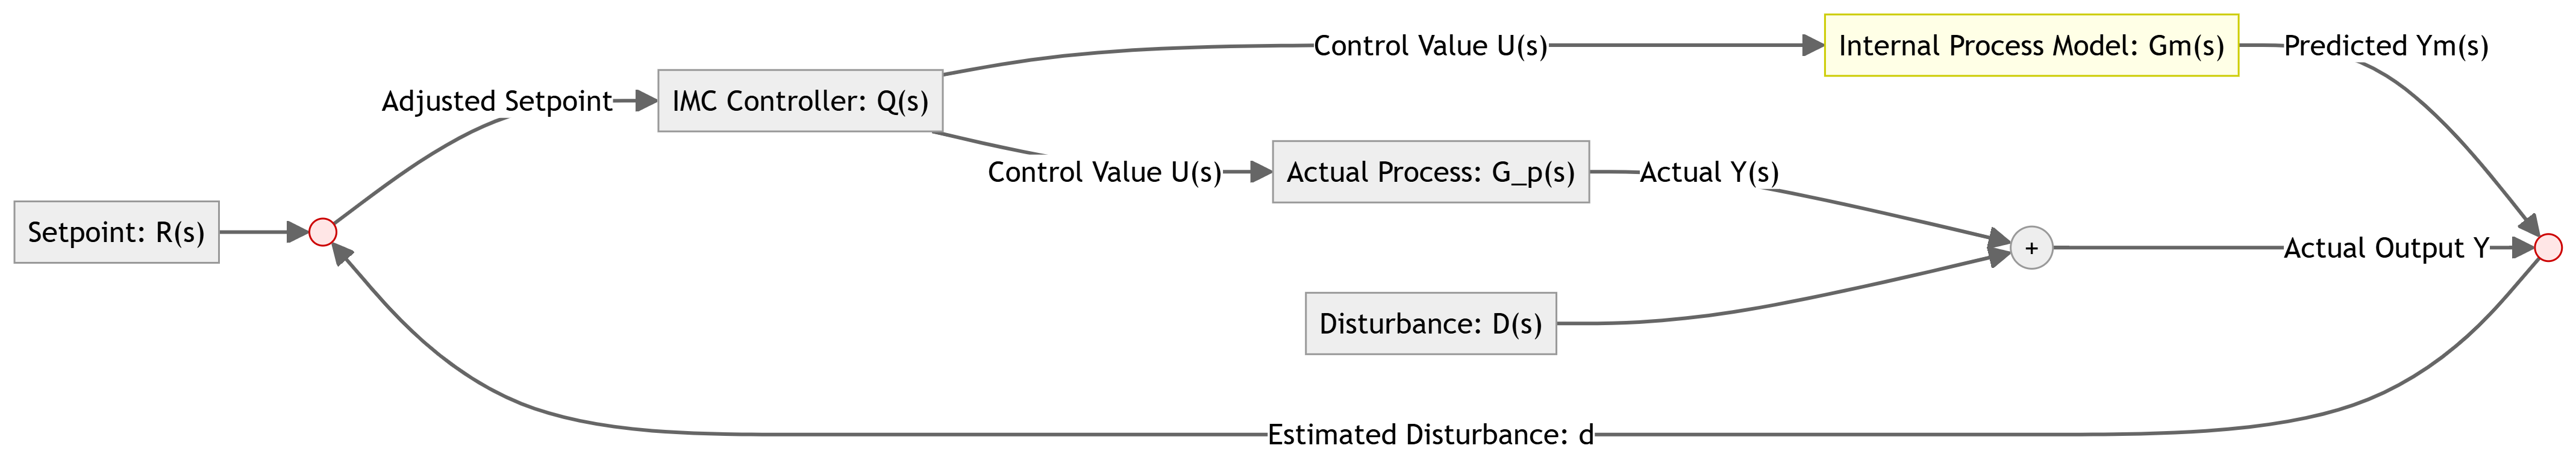
\includegraphics[width=0.75\textwidth,height=0.32\textheight,keepaspectratio]{../Images/chapter_04/imc_block.png}
\caption{Internal Model Control (IMC) Block Diagram}
\end{figure}


\section{Section 4: Solved Exam One-Liners (Active Recall Database)}

\begin{itemize}
  \item \textbf{Q1. What is the operating frequency of an ultrasonic sensor?}
  \item \textit{Answer:} \textbf{10–65 kHz}
  \item \textbf{Q2. The primary sensing element of the pressure thermometer is \_\_\_\_\_\_\_.}
  \item \textit{Answer:} \textbf{Pressure bulb filled with a liquid}
  \item \textbf{Q3. Thermocouples generate output voltage according to the \_\_\_\_\_\_\_.}
  \item \textit{Answer:} \textbf{Seebeck effect}
  \item \textbf{Q4. Touch screen devices use which sensor?}
  \item \textit{Answer:} \textbf{Capacitive sensors}
  \item \textbf{Q5. What is the purpose of a pressure gauge in a boiler plant?}
  \item \textit{Answer:} \textbf{To measure pressure and display it}
  \item \textbf{Q6. State the cause for using starters with D.C. motors.}
  \item \textit{Answer:} \textbf{To limit the high starting current}
  \item \textbf{Q7. The span of the pneumatic signal used in industry is \_\_\_\_\_\_\_.}
  \item \textit{Answer:} \textbf{3-15 psi}
  \item \textbf{Q8. The gauge factor of a strain gauge indicates its \_\_\_\_\_\_\_.}
  \item \textit{Answer:} \textbf{Sensitivity}
  \item \textbf{Q9. Cohen-Coon tuning rules are used for \_\_\_\_\_\_\_ systems.}
  \item \textit{Answer:} \textbf{Processes with time-lag and self-regulation}
  \item \textbf{Q10. What type of controller is used for the elimination of offset?}
  \item \textit{Answer:} \textbf{Integral controller (I-controller)}
  \item \textbf{Q11. The Ziegler-Nichols tuning method is used for \_\_\_\_\_\_\_.}
  \item \textit{Answer:} \textbf{Processes with time-lag and self-regulation}
  \item \textbf{Q12. The derivative mode (D controller) is also known as \_\_\_\_\_\_\_.}
  \item \textit{Answer:} \textbf{Rate controller}
  \item \textbf{Q13. If the proportional band of an electronic PID controller is set at 10, then what is the proportional gain ($K_c$)?}
  \item \textit{Answer:} \textbf{Proportional gain $K_c = 100 / PB = 100/10 = 10$}
  \item \textbf{Q14. The quarter-amplitude decay ratio is basically a design criterion specified by the Ziegler-Nichols method which implies that the amplitude of an oscillation must be reduced by a factor of \_\_\_\_\_\_\_.}
  \item \textit{Answer:} \textbf{1/4}
  \item \textbf{Q15. A summing amplifier block followed by an inverter block represents a \_\_\_\_\_\_\_ controller.}
  \item \textit{Answer:} \textbf{PI/PID controller} (when integrating and proportional resistors are configured)
  \item \textbf{Q16. What are the advantages of a pneumatic controller?}
  \item \textit{Answer:} \textbf{Simple construction, explosion-proof/safe in hazardous areas, high power output}
  \item \textbf{Q17. Which of the following controllers has the maximum offset? (a) P-controller (b) P-I controller (c) P-I-D controller (d) P-D controller}
  \item \textit{Answer:} \textbf{(a) P-controller}
  \item \textbf{Q18. In an electronic Integral controller, if the resistance and capacitance values are both doubled, then the controller response time will be \_\_\_\_\_\_\_ and the controller gain will be \_\_\_\_\_\_\_.}
  \item \textit{Answer:} \textbf{Doubled, quartered} (since integration time constant $\tau_I = RC$ is quadrupled)
  \item \textbf{Q19. If the Proportional Band (PB) of a P-controller is very wide, then the system response is \_\_\_\_\_\_\_.}
  \item \textit{Answer:} \textbf{Slow (and has high offset)}
  \item \textbf{Q20. The function of reset action in a process controller is to \_\_\_\_\_\_\_.}
  \item \textit{Answer:} \textbf{Eliminate offset (steady-state error)}
  \item \textbf{Q21. Which controllers do not show a continuous action?}
  \item \textit{Answer:} \textbf{Digital controllers} (discrete-time action)
  \item \textbf{Q22. What is the transfer function of a dead-time element?}
  \item \textit{Answer:} \textbf{$G(s) = e^{-s T_d}$}
  \item \textbf{Q23. Provide an example of a self-regulating system.}
  \item \textit{Answer:} \textbf{Liquid level in a tank with constant gravity outflow}
  \item \textbf{Q24. Which control valve is used for pressure control?}
  \item \textit{Answer:} \textbf{Globe valve} (often used for throttling control)
  \item \textbf{Q25. Database management and decisions regarding production are handled in which level of the DCS structure?}
  \item \textit{Answer:} \textbf{Level 3 (Production control/Management level)}
  \item \textbf{Q26. What are the components of a SCADA system?}
  \item \textit{Answer:} \textbf{MTU (Master Terminal Unit), RTU (Remote Terminal Unit) or PLCs, Communication Network, HMI (Human Machine Interface)}
  \item \textbf{Q27. When a control valve plug is fully connected to the \_\_\_\_\_\_\_, then it is fully closed.}
  \item \textit{Answer:} \textbf{Valve seat}
  \item \textbf{Q28. A cascade controller is used when the process shows \_\_\_\_\_\_\_.}
  \item \textit{Answer:} \textbf{Slow response and large time lag (multiple capacities)}
  \item \textbf{Q29. State the load disturbances in the feed-forward control strategy of a simple heat exchanger.}
  \item \textit{Answer:} \textbf{Inlet flow rate, inlet temperature, and fluid composition}
  \item \textbf{Q30. Which control scheme is known as anticipatory control?}
  \item \textit{Answer:} \textbf{Feed-forward control}
  \item \textbf{Q31. When should Cascade Control be used?}
  \item \textit{Answer:} \textbf{When there are significant secondary disturbances that affect the primary loop}
  \item \textbf{Q32. The response of Feed-forward control is \_\_\_\_\_\_\_ than Feedback control.}
  \item \textit{Answer:} \textbf{Faster (proactive/anticipatory)}
  \item \textbf{Q33. A ratio control system is a special type of \_\_\_\_\_\_\_ control system.}
  \item \textit{Answer:} \textbf{Feed-forward control system}
  \item \textbf{Q34. The purpose of ratio control is to \_\_\_\_\_\_\_.}
  \item \textit{Answer:} \textbf{Maintain a constant ratio between two process variables (e.g., fuel and air ratio)}
\end{itemize}
